\renewcommand{\lastmod}{10. September 2024}
\renewcommand{\chapterauthors}{Markus Lippitz}

\chapter{Elementare Anregungen in Molekülen}



\goal{By the end of this chapter, you should be able to draw, calculate and align a ray's path through an optical system.}



\section{Overview}

s.a. Demtröder 3, Kap. 9


11.1 Rotation: IR Absorption [6] 1	

11.2 Schwingung: IR Absorption [6] 2	 

11.3 Schwingung: Raman Streuung 3	 

11.4 Elektronische Anregung: Absorption 4	 

11.5 Elektronische Anregung: Fluoreszenz 5	 



%%%%%%%%%%%%%%%%%%%%%%%%%%%%%%%%%%%%%%%%%%%%%%%%%
%%%%%%%%%%%%%%%%%%%%%%%%%%%%%%%%%%%%%%%%%%%%%%%%%


\section{Ziele}

\begin{itemize}
\item Sie können die Phänomene erklären und durch einfache Modelle beschreiben, die in den  dielektrischen Eigenschaften von Molekülen zu finden sind, beispielsweise diese dielektrische Funktion von Wasser (siehe auch Pluto-Skript\pluto{water}).


\end{itemize}

\begin{figure}
\inputtikz{\currfiledir fig_water}
\caption{Dielektrische Funktion $\epsilon = \epsilon' - i \, \epsilon''$ von flüssigem Wasser (\cite{Segelstein_water} via 
\href{https://refractiveindex.info/?shelf=main&book=H2O&page=Segelstein}{refractiveindex.info}). Der niederfrequente Bereich unterhalb von $\bar{\nu} = 30$~cm$^{-1}$ ist um den Faktor 20 reduziert dargestellt.
\label{fig:diel_water}}

%D. J. Segelstein. The complex refractive index of water, Master Thesis (1981)
%https://refractiveindex.info/?shelf=main&book=H2O&page=Segelstein
% http://hdl.handle.net/10355/11599 
\end{figure}

\section{Wie misst man das ?}

Das oben gezeigte Spektrum überdeckt mehr als 6 Größenordnungen im Frequenzbereich und ist mit einem einzigen Gerät nicht  messbar. Die niedrigsten Frequenzen liegen im Bereich von Mikrowellen, benutzt also Techniken aus dem Radio- und Radar-Bereich. Der mittlere Frequenzbereich ist infrarotes Licht, der hohe sichtbares bis ultraviolettes Licht. Wir werden die verschiedenen spektroskopischen Methoden in den folgenden Kapiteln besprechen.


Die Wellenzahl $\bar{\nu} = 1 / \lambda =\nu / c =  E / (h c)$ (eigentlich immer angegeben in der Einheit 1/cm) ist eine Maß für die  \emph{Frequenz} oder \emph{Energie}. Dieses Maß in der Spektroskopie sehr weit verbreitet ist, weil es proportional zur Energie ist (und damit das Reziproke der Wellenlänge umgeht), aber gleichzeitig nahe an der praktischen, intuitiven Größe 'Wellenlänge'.



\begin{questions} 
\item Wo in  Abbildung  \ref{fig:diel_water} ist der sichtbare Spektralbereich, wo die Frequenz von Radio Mainwelle?
\end{questions}


\section{Erinnerung an die Elektrostatik }

Es gibt die Maxwell-Gleichungen in einer mikroskopischen Form und in einer makroskopischen Form.
%
\begin{align}
\text{mikroskopische Form} & &
\text{makroskopische Form} \nonumber \\
%
%\text{Gaußsches Gesetz} &
 \nabla\cdot\mathbf{E}= \frac{\rho}{\epsilon_0} & &
 \nabla\cdot\mathbf{D}= \rho_{\text{frei}} \\
%
%\text{Gaußsches Gesetz für Magnetfelder }&
\mathbf\nabla\cdot\mathbf{B}=0
 & &
\mathbf\nabla\cdot\mathbf{B}=0 \\
%
%\text{Induktionsgesetz} &
\mathbf\nabla\times\mathbf{E}=-\frac{\partial\mathbf{B}}{\partial t}  
& &
\mathbf\nabla\times\mathbf{E}=-\frac{\partial\mathbf{B}}{\partial t} \\
%
%\text{Erweitertes Durchflutungsgesetz} &
\mathbf\nabla\times\mathbf{B}= \mu_0\mathbf{j}+\mu_0\epsilon_0\frac{\partial\mathbf{E}}{\partial t}  & &
\mathbf\nabla\times\mathbf{H}= \mathbf{j}_{\text{frei}}+\frac{\partial\mathbf{D}}{\partial t}
\end{align}
%
Die makroskopische Form berücksichtigt dabei die Gegenwart von Medien, in dem die Größen dielektrische Verschiebung $\mathbf{D}$ und magnetische Feldstärke $\mathbf{H}$ eingeführt werden. Dies ist einerseits historisch bedingt, weil zur Zeit Maxwells der mikroskopische Aufbau der Materie noch unbekannt war. Andererseits ist es aber auch heute hilfreich, nicht alle Details der mikroskopischen Struktur der Materie explizit berücksichtigen zu müssen, sondern durch gemittelte, makroskopische Parameter beschreiben zu können.

Besonders deutlich wird dies bei der Unterscheidung zwischen freien Ladungen und Polarisationsladungen.  Vom modernen, mikroskopischen Standpunkt her trennt man die Elektronen in zwei Gruppen: von außen beispielsweise auf einen Kondensator aufgebrauchte (= freie) und durch Verschiebung der schon vorhandenen Elektronen in einem Dielektrikum an einem Ort neu hinzukommende Polarisationsladung. Letztere Verschiebung ist eine Konsequenz der Anwesenheit der freien Ladungen.

Wenn wir ein Stück dielektrische Materie in einen Plattenkondensator halten, dann bewegt das elektrische Feld $\mathbf{E}$ des Kondensators die Ladungsträger der Ladung $q$ in der Materie um  die Distanz $\Delta  \mathbf{x}$ von der neutralisierenden Gegenladung $-q$ weg. Dadurch entsteht dadurch ein Dipolmoment $\mathbf{p} = q \Delta \mathbf{x}$. Oft werden Dipolmomente in der Einheit Debye angegeben ($1 D = 3{,}33564 \cdot 10^{-30}$ C  m). Ein Elektron im Abstand von 1~\AA\ von einem Proton produziert ein Dipolmoment von etwa 4.8~D. Bei $N$ Molekülen (Ladungsträgerpaaren) pro Volumen ergibt sich eine makroskopische Polarisation $\mathbf{P}$ zu
\begin{equation}
\mathbf{P} = N \, q \, \Delta \mathbf{x} = f(\mathbf{E}) \quad .
\end{equation}
Der Zusammenhang zwischen angelegtem externen Feld $\mathbf{E}$ und resultierende 
Polarisation $\mathbf{P}$ hängt ganz entscheidend vom mikroskopischen Aufbau der Materie ab. Alle Methoden der Spektroskopie vermessen diesen Zusammenhang. Oft wird er als 
\begin{equation}
 \mathbf{P} =  (\epsilon - 1) \, \epsilon_0 \, \mathbf{E} = \epsilon_0 \,\chi \, \mathbf{E} 
 \label{eq:diel_p_lin}
\end{equation}
geschrieben, mit der relativen Permittivität\sidenote{Vorsicht, hier gibt es verschiedene Schreibweisen. Ich benutze die Form $D = \epsilon \epsilon_0 E$, mit einheiten-freiem $\epsilon$. Manchmal findet man $\epsilon_0 \epsilon_r$, manchmal auch nur $\epsilon$.} $\epsilon$ bzw. der elektrischen Suszeptibilität $\chi$. Dies ist aber nur eine Näherung. In allgemeiner Form ist der Zusammenhang
\begin{equation}
\mathbf{P}  = \epsilon_0 \left( \chi^{(1)} \mathbf{E} + \chi^{(2)} : \mathbf{E}  \mathbf{E} +  \chi^{(3)} \, \vdots  \, \mathbf{E}  \mathbf{E}  \mathbf{E}  + \dots \right) \quad .
\end{equation}
Zum einen muss der Polarisation-Vektor nicht unbedingt in die Richtung des elektrischen Feldes zeigen. Dies macht die $\chi^{(n)}$ zu Tensoren $(n+1)$ter Stufe und führt beispielsweise zu Doppelbrechung. Zum anderen muss der Zusammenhang zwischen Feld und Polarisation nicht unbedingt linear sein, wodurch verschieden Taylor-Koeffizienten notwendig werden. Dies ist Thema der nichtlinearen Optik.

In diesem Kapitel betrachten wir allgemeine, einfache Aussagen über die dielektrische Funktion $\epsilon$.
Das Thema der folgenden Kapitel ist, wie man aus Vermessung von $\epsilon$ Aussagen über den Aufbau  von Molekülen, insbesondere über die Parameter des Bindungspotentials machen kann.





\section{Unpolare Moleküle: Verschiebungspolarisation}

Betrachten wir zunächst unpolare Moleküle, also solche, die kein permanentes Dipolmoment  besitzen\sidenote{siehe auch \cite[Kapitel 3]{Haken_wolf_II}}. Dies sind insbesondere zentro-symmetrische Moleküle wie \ch{H2}, \ch{O2}, \ch{N2}, \ch{CCl4}. Aber ein externes angelegtes elektrisches Feld verschiebt die Ladungen\sidenote{Elektronen gegenüber Kernen, aber auch Kationen gegenüber Anionen} relativ zueinander und induziert ein Dipolmoment
\begin{equation}
 \mathbf{p}_\text{ind} = \alpha \, \mathbf{E}_\text{lokal}
\end{equation}
mit der Polarisierbarkeit $\alpha$ und dem Feld am Ort der Ladungen $\mathbf{E}_\text{lokal}$.

\paragraph{Verdünntes molekulares Gas} Wenn die Moleküle sehr weit voneinander entfernt sind, beispielsweise in einem verdünnten Gas, dann haben die anderen Moleküle keinen Einfluss auf das Feld, das das eine betrachtete Molekül sieht. Das lokale Feld ist gleich dem externen Feld.
 Damit gilt
\begin{equation}
 \mathbf{P} = N \, \alpha \, \mathbf{E}_\text{lokal} =  \frac{\rho \, N_A } {M} \, \alpha \, \mathbf{E} \label{eq:diel_pind}
\end{equation}
mit der Teilchenzahldichte $N$, dem Molekulargewicht $M$, der (Masse-)DIchte $\rho$ und Avogadro-Konstanten $N_A$. Mit Gl \ref{eq:diel_p_lin} erhält man so
\begin{equation}
 \epsilon = 1 +  \frac{\rho \, N_A } {M \, \epsilon_0} \, \alpha   \quad .
\end{equation}
Man kann also die dielektrische Konstante $\epsilon$ messen und die die Polarisierbarkeit $\alpha$ bestimmen. Oft wird $\alpha' = \alpha / 4 \pi \epsilon_0$ angegeben, was die Einheit eines Volumens hat, das Polarisierbarkeitsvolumen. Beides sind Tensoren, also richtungsabhängig.

\begin{marginfigure}
\begin{tabular}{llll}
 & $\braket{\alpha'} $ & $\alpha'_\perp$ & $\alpha'_\parallel$ \\
\ch{H2} & 0.79 & 0.61 & 0.85 \\
\ch{C6H6} & 10.3 & 6.7 & 12.8 
\end{tabular}
\caption{Polarisierbarkeitsvolumen einiger Moleküle (in Einheiten von $10^{-30}$ m$^3$.)}
\end{marginfigure}

\paragraph{Flüssigkeiten} Bei höherer Dichte, also beispielsweise in einer Flüssigkeit, muss man die anderen, ebenfalls polarisierten Moleküle berücksichtigen. Verschiedene Methoden sind dabei möglich\footcite{Parson}, die unter dem Stichwort \emph{local field correction} zusammengefasst sind.

Wir betrachten hier die Lorentz-Methode. Alle Moleküle zusammen werden als  ein homogenes Medium mit der  dielektrische Konstante $\epsilon$  angesehen. Aus diesem Medium schneidet man eine Kugel aus, die gerade das einzelne, zu betrachtende Molekül umschließt. In die so entstandene Aushöhlung setzt man das Molekül in Vakuum, also wieder in einem sehr verdünnten Gas. Das externe elektrische Feld induziert eine Polarisation  $\mathbf{P}$, nur kennen wir deren Größe noch nicht. Diese Polarisation bewirkt  Oberflächenladungen am Rand der Kugel, die das lokale Feld in der Kugel modifizieren:
\begin{equation}
\mathbf{E}_\text{lokal} = \mathbf{E} + \frac{1}{3 \, \epsilon_0} \, \mathbf{P} \quad . \label{eq:diel_local_field_correction}
\end{equation}
Damit können wird dann mit Gl.\ref{eq:diel_pind} das induzierte Dipolmoment berechnen
\begin{align}
 \mathbf{P} = N \, \alpha \, \mathbf{E}_\text{lokal} =&
   \frac{\rho \, N_A }{M} \, \alpha \, \left( \mathbf{E} + \frac{1}{3 \, \epsilon_0} \, \mathbf{P} \right)   \\
   =&
     \frac{\rho \, N_A }{M} \, \alpha \, \left( \frac{1}{\epsilon_0 ( \epsilon -1)}\mathbf{P} + \frac{1}{3 \, \epsilon_0} \, \mathbf{P} \right)  \quad .
\end{align}
 $\mathbf{P}$ kürzt sich heraus und wir erhalten durch Umstellen die 
\emph{Clausius-Mosotti-Gleichung}
 \begin{equation}
 \frac{\epsilon - 1}{\epsilon + 2} \frac{M}{\rho} = \frac{1}{3} \frac{N_A}{\epsilon
_0} \, \alpha \quad .\label{eq:diel_Clausius-Mosotti}
 \end{equation}
 Das bemerkenswerte ist, dass wir die makroskopischen, messbaren Größen $\epsilon$,$M$, $\rho$ mit der molekularen Polarisierbarkeit $\alpha$ verknüpfen können. Durch einfache Messungen beispielsweise einer Flüssigkeit können wir eine mikroskopische Aussage über das Molekül machen.
 
Bisher haben wir immer quasi-statische elektrische Felder angenommen.  Die Clausius-Mosotti-Gleichung findet aber auch bei optischen Feldern eine Entsprechung. Der Brechungsindex ist $n = \sqrt{\epsilon \, \mu}$ mit der Permeabilitätskonstanten $\mu$. Diese ist im optischen Frequenzbereich aber sehr nahe an eins, also $n = \sqrt{\epsilon }$. Damit wird Gl. \ref{eq:diel_Clausius-Mosotti} zu 
  \begin{equation}
 \frac{n^2 - 1}{n^2 + 2} \frac{M}{\rho} = \frac{1}{3} \frac{N_A}{\epsilon
_0} \, \alpha_\text{optisch} \quad . \label{eq:diel_Lorentz_Lorenz}
 \end{equation}
 Diese Gleichung heißt Lorentz-Lorenz-Gleichung und beschreibt die \emph{optische Polarisierbarkeit} $\alpha_\text{optisch}$. Wie wir weiter unten sehen werden, unterscheiden sich $\alpha$ und  $\alpha_\text{optisch}$ bzw. $\epsilon(\nu \approx 0)$ und $\epsilon(\nu \approx 300 \text{ THz})$ deutlich.
 
 
\begin{questions} 
\item Blättern Sie in Ihrem Skript / Lehrbuch zur Elektrodynamik und schauen sich die Herleitung von Gl. \ref{eq:diel_local_field_correction} an.
\end{questions}
 
\section{Polare Moleküle: Orientierungspolarisation}
 
Polare Moleküle wie beispielsweise \ch{H2O} oder \ch{HCl} besitzen ein Dipolmoment $\mathbf{p}$, auch wenn kein externes Feld angelegt wird. Wenn dann doch ein Feld angelegt wird, dann verschieben sich nicht nur die Ladungen wie im letzten Abschnitt, sondern der schon vorhandene Dipol und damit das Molekül richtet sich im externen Feld aus. Dieser Ausrichtung stehen thermische Fluktuationen entgegen. Das entstehende Gleichgewicht ähnlich einer Boltzmann-Verteilung hängt vom Verhältnis der Energie des Dipols im Feld $\mathbf{p} \cdot \mathbf{E}$ und der thermischen Energie $k_B \, T$ ab. 

\paragraph{Verdünnte Gase} Wenn wir zunächst wieder den Einfluss der anderen Moleküle vernachlässigen, dann ist die makroskopische Orientierungspolarisation $\mathbf{P}_\text{or}$ die Vektor-Summe über die einzelnen statischen Dipolmomente $ \mathbf{p}$. Sei $\theta$ der Winkel zwischen dem einzelnen Dipolmoment und dem externen Feld, dann lässt sich dies schreiben als
\begin{equation}
P_\text{or} = N \, p \, \braket{ \cos \theta}  \quad ,
\end{equation}
wobei die spitze Klammer das Ensemble-Mittel bezeichnen. Statistische Rechnungen ergeben
 \begin{equation}
P_\text{or} = N \, p \, L \left( \frac{p \, E}{k_B \, T} \right)
\end{equation}
mit der Langevin-Funktion $L(x)$
\begin{equation}
L(x) = \coth x - \frac{1}{x} \approx \frac{x}{3} \quad \text{für} \quad x \ll 1 \quad .
\end{equation}
Damit werden die Orientierungspolarisation und die dielektrische Konstante
\begin{equation}
\mathbf{P}_\text{or} = N \, \frac{|\mathbf{p} |^2}{3 \, k_B \, T} \, \mathbf{E}  \quad \text{und} \quad \epsilon = 1 + N \, \frac{|\mathbf{p} |^2}{3\, \epsilon_0 \, k_B \, T} \quad .
\end{equation}
Dies ist sowohl vom Formalismus als auch vom Ergebnis identisch zum Curie-Gesetz für paramagnetische Materialien. Die Orientierungspolarisation ist also temperaturabhängig, im Gegensatz zur Verschiebungspolarisation.

\paragraph{Verschiebungs- und Orientierungs-Polarisation} Beide Polarisationen addieren sich und gehen gemeinsam in die dielektrische Konstante ein:
\begin{equation}
\mathbf{P}  = \mathbf{P}_\text{ind} + \mathbf{P}_\text{or} = \left( \epsilon - 1 \right) \, \epsilon_0 \, \mathbf{E}  \quad .
\end{equation}
Auch in dichten Medien kann man analog zur Verschiebungspolarisation eine Korrektur für das lokale Feld einführen. Die Clausius-Mosotti-Gleichung wird, wenn man beide Polarisationen zusammen nimmt, zur Debye-Gleichung
 \begin{equation}
 \frac{\epsilon - 1}{\epsilon + 2} \frac{M}{\rho} = \frac{1}{3} \frac{N_A}{\epsilon
_0} \,  \left( \alpha  + \frac{|\mathbf{p} |^2}{3 \, k_B \, T}  \right) \quad .
 \end{equation}
 
 
\section{Frequenzabhängigkeit der dielektrische 'Konstanten' }
 
Bisher haben wir nur statische elektrische Felder betrachtet. Nun wollen wir auch Licht, also elektromagnetische Felder bei  höheren, optischen Frequenzen  betrachten. Die dielektrische 'Konstante' $\epsilon$ ist dann nicht mehr konstant, sondern eine dielektrische Funktion der Frequenz, also $\epsilon(\nu)$. Welche Frequenzen sind 'hoch'? Bei welchen Frequenzen erwarten wir, dass Verschiebungs- und Orientierungspolarisation nicht mehr mit kommen?

\paragraph{Orientierungspolarisation} Die Orientierung des Moleküls im Feld ist eine Drehbewegung. Diese Bewegungen werden bei der Rotationsspektroskopie im nächsten Kapitel detaillierter behandelt werden. Hier greifen wir vor. Der Drehimpuls $L$ ist in der Quantenmechanik quantisiert. Sei
\begin{equation}
1 \hbar = L = J \, \omega = m_\text{red} \, R^2 \, \omega
\end{equation}
mit dem Trägheitsmomnet $J$, der Kreisfrequenz $\omega$ und der reduzierten Masse 
 $m_\text{red}$ sowie dem Bindungsabstand $R$ in einem angenommenen zwei-atomigen Molekül. Für das Molekül HCl gilt $R = 1.28$~\AA\ und $m_\text{red} \approx m_H = 1$~u. Damit ergibt sich eine Frequenz $\nu = 628$ GHz, also im Mikrowellen-Bereich. Oft wird dies auch geschrieben als Wellenzahl $\bar{\nu} = 1 /\lambda \approx 10$~cm$^{-1}$.
 
\paragraph{Verschiebung der Kerne} Bei der Verschiebungspolarisation können sich zunächst einmal die Kerne bzw. Ionen gegeneinander bewegen. Dies ist Thema der Schwingungsspektroskopie, und wieder greifen wir vor. Zwei Atome seien im Gleichgewicht  im Bindungs-Abstand $R_0$. Wir nehmen an, die Rückstellkraft in diesem Gleichgewicht sein allein die Coulomb-Kraft des einen Kerns auf den anderen, also 
\begin{equation}
F = \frac{1}{4 \pi \epsilon_0} \, \frac{e^2}{R^2} \quad .
\end{equation}
Die Federkonstante $k$ ist dann die Ableitung dieser Kraft nach $R$. Für das Molekül HCl mit einem Gleichgewichts-Abstand $R_0 = 1.2$~\AA\ ergibt sich $k = 220$~N/m. Die Eigenfrequenz der Schwingung  ist $\nu = (1/2\pi) \, \sqrt{k/m_\text{red}} = 58$~THz mit der reduzierten Masse von oben. Dies entspricht einer Wellenlänge von $\lambda = 5.12$~\textmu m, also im Infraroten, und einer Wellenzahl $\bar{\nu} = 2000$~cm$^{-1}$.

\paragraph{Verschiebung der Elektronenwolke} Wenn es zu einer Resonanz in der Verschiebung der Elektronenwolke kommt, dann entspricht dies einer elektronischen Anregung, also einem quantenmechanischen Übergang zwischen zwei Elektronen-Orbitalen. Auch dies wird uns in einem der folgenden Kapitel beschäftigen. Wir schätzen hier die Übergangsenergie analog zu atomaren Übergängen ab
\begin{equation}
  h \nu = hc \, R_H \, \left( \frac{1}{n^2} - \frac{1}{m^2} \right) \quad .
\end{equation}
Für Atome liegt die Frequenz $\nu$ im Bereich von $10^{15}$~Hz $= 1$~PHz. Bei Molekülen liegt sie etwas niedriger, also $\nu \approx 10^{14} \cdots 10^{15}$~Hz, also $100 \cdots 1000$~THz.


\section{Lorentz-Oszillator-Modell}


\begin{marginfigure}
\inputtikz{\currfiledir lorentz_oszillator}

\caption{Frequenzabhängigkeit des Real- und Imaginärteils des Lorentz-Oszillators. Real- und  Imaginärteil des komplexwertigen Brechungsindex $\tilde{n}$ sehen qualitativ gleich aus. \label{fig:diel_lorentz}}
\end{marginfigure}

Alle oben diskutieren Phänomene sind Resonanzen. Das Lorentz-Oszillator-Modell ist ein einfaches Modell, mit dem die Frequenzabhängigkeit der dielektrischen Funktion in der Nähe solcher Resonanzen beschrieben werden kann. In einem gedämpften harmonischen Oszillator (Masse $m$, Dämpfungskonstante $\gamma$, Eigenfrequenz $\omega_0$) wird die Masse durch ein periodisches elektrisches Feld (Amplitude $E_0$, Frequenz $\omega$) um $x$ ausgelenkt, da die Masse eine Ladung $e$ trägt. Alles zusammen
\begin{equation}
 m \ddot{x} +  \gamma \dot{x} + m \omega_0^2  x = e E_0 e^{+ i \omega t} \quad .
\end{equation}
Die stationäre Lösung dieser Differentialgleichung ist
\begin{equation}
 x(t) =  \frac{e \, E_0}{m (\omega_0^2  - \omega^2) + i \gamma \omega} \, e^{+ i \omega t} \quad .
\end{equation}
Die makroskopische Polarisation $P$ ist die Summe über alle mikroskopische Polarisationen, also
\begin{equation}
P(t) = N \, e \,x(t) =  (\epsilon -1 ) \epsilon_0 \, E_0 e^{+ i \omega t}
= \chi \epsilon_0 E(t) \quad .
\end{equation}
Damit ergibt sich die dielektrische Funktion
\begin{equation}
\epsilon(\omega) = 1 + N \alpha = 1 +\frac{N e^2}{\epsilon_0} \frac{1}{m (\omega_0^2  - \omega^2) + i \gamma \omega} = \epsilon' - i \epsilon'' \quad .
\end{equation}
Man beachten das per Konvention negative Vorzeichen des Imaginärteils $\epsilon''$. Explizit sind Real- und Imaginärteil
\begin{align}
 \epsilon' = & 1 + \frac{N e^2}{\epsilon_0} \frac{ m (\omega_0^2  - \omega^2)}{m^2 (\omega_0^2  - \omega^2)^2 +  \gamma^2 \omega^2}  \\
  \epsilon'' = &  \frac{N e^2}{\epsilon_0} \frac{ \gamma \omega }{m^2 (\omega_0^2  - \omega^2)^2 +  \gamma^2 \omega^2}  \quad .
\end{align}
Für den  komplexwertige\sidenote{Oft wird nicht zwischen $n$ und $\tilde{n}$ unterschieden und $n$ selbst ist komplexwertig.} Brechungsindex\sidenote{Die hier benutzte Konvention der Vorzeichen ist die in der Physik übliche, ausgehend von der Zeitabhängigkeit $e^{+ i \omega t}$. In der eher ingenieurwissenschaftlichen Literatur findet sich aber genauso oft auch die Zeitabhängigkeit $e^{- i \omega t}$. Dies führt zu komplex-konjugierten Gleichungen. } $\tilde{n} = n - i k$ gilt
\begin{align}
 \epsilon = & \tilde{n}^2 = (n - i k)^2 \\
  \epsilon' =& n^2 - k^2 \\
 \epsilon'' = & 2 n k \quad .
\end{align}
Dabei beschreibt $k$ die Dämpfung und $n$ die Dispersion, also die Variation der effektiven Wellenlänge in der Nähe einer Resonanz:
\begin{equation}
E(t,z) = E_0 \, e^{i \omega (t - \frac{z}{c}(n - i k))} = 
 E_0 \, e^{ - \frac{\omega}{c} k z}  
 \, e^{i \omega (t - \frac{z}{c/n} )}  \quad .
\end{equation}

Wenn in einem Medium mehrere Resonanzen vorhanden sind, so addieren sich die Suszeptibilitäten:
\begin{equation}
\epsilon(\omega)_\text{ges} = 1 + \chi(\omega)_\text{elec} +  \chi(\omega)_\text{ion}  + \chi(\omega)_\text{orient} \quad .
\end{equation}

\begin{marginfigure}
\inputtikz{\currfiledir multiple_lorentz_oszillator}

\caption{Addition der Suszeptibilitäten. \label{fig:diel_multiple_lorentz}}
\end{marginfigure}

Für Fensterglas liegt die elektronische Resonanz im Ultravioletten. Sichtbares Licht ist also im Frequenzbereich etwas unterhalb dieser Resonanz. Die sogenannte 'normale' Dispersion des Brechungsindex (ansteigend mit fallender Wellenlänge / steigender Frequenz) rührt gerade von dem Anstieg der dielektrischen Funktion zur elektronischen Resonanz hin her.


\begin{questions} 
\item Stellen Sie analog zu Abbildung \ref{fig:diel_lorentz} die Frequenzabhängigkeit der Komponenten des Brechungsindexes, also  von $n$ und $k$ dar.

\item Nähern sie den Real- und Imaginär-Teil von $\epsilon$ in der Nähe der Resonanz bei  $\omega_0$ als Funktion von $\Delta \omega = \omega - \omega_0$. Im Fall des Realteils ist nur der Bereich $| \Delta \omega | \gg \gamma/m$ interessant.
\end{questions}

\section{Die Kramers-Kronig-Relationen}

Wir haben bisher den Zusammenhang zwischen dem angelegten externen Feld $E(t)$ und der entstehenden Polarisation $P(t)$ eigentlich nur für 'monochromatische' Felder der Art $\exp(i \omega t)$ diskutiert, also für eine genau bestimmte Frequenz $\omega$:
\begin{equation}
P(t) = \chi(\omega) \epsilon_0 E(t) \quad \text{für} \quad E(t) = E_0 e^{i \omega t} \quad .
\end{equation}
Daraus ergab sich dann die Frequenzabhängigkeit von $\chi(\omega)$ Wir können dies verallgemeinern für einen beliebigen zeitlichen Verlauf des Feldes  $E(t)$. Die Suszeptibilität ist nämlich die  \emph{Impulsantwort} des Materials, sozusagen das Gedächtnis:
\begin{equation}
P(t) = \epsilon_0 \int_{-\infty}^{+\infty} \chi( \Delta t = t - t') \, E(t') \, dt' \quad \text{für} \quad E(t) = \text{beliebig} \quad .
\end{equation}
Die Polarisation $P$ jetzt, also zum Zeitpunkt $t$ hängt vom elektrischen Feld zu allen anderen Zeiten $t'$ ab. Wie stark die Felder eingehen, hängt nur vom zeitlichen Abstand $\Delta t$ ab. Die Kausalität verlangt, dass die Polarisation 'jetzt' nicht von Feldamplituden in der Zukunft abhängen darf. $\chi( \Delta t = t - t' < 0) $ muss daher Null sein. Damit ist die Suszeptibilität $\chi( \Delta t ) $ zwar komplexwertig, aber über die eine Hälfte des Zeitstrahls bekannt und zu Null festgelegt. Dies hat Konsequenzen für die Fouriertransformation, also für $\chi(\omega)$.

Diese Konsequenzen lassen sich mit Hilfe der Funktionentheorie herleiten\sidenote{siehe auch Anhang A von \cite{Yariv1989}} und sind die Kramers-Kronig-Relationen. Es besteht folgender Zusammenhang zwischen Real- ($\chi'$) und Imaginärteil  ($\chi''$) der Suszeptibilität, wenn dieser der Kausalität gehorcht:
\begin{align}
 \chi'(\nu) = & \frac{2}{\pi} \, CH \int_0^\infty \frac{s  \, \chi''(s)}{s^2 - \nu^2} \, ds \\
 \chi''(\nu) = & \frac{2}{\pi}\,  CH \int_0^\infty \frac{\nu \, \chi'(s)}{\nu^2 - s^2} \, ds  \quad .
 \label{eq:diel_KK}
\end{align}
$CH$ kennzeichnet dabei das Cauchy'sche Hauptwertintegral. Ähnliche Beziehung existieren auch für $\chi(\omega)$ und $\epsilon(\omega)$ sowie für alle anderen Größen, die der Kausalität unterliegen.

Es reicht also im Prinzip aus, den Realteil der Suszeptibilität $\chi(\omega)$ zu messen, um daraus den Imaginärteil und somit die komplette komplexwertige Funktion zu bestimmen. Leider laufen die Integrale in Gl~\ref{eq:diel_KK} aber über den ganzen Frequenzbereich von Null bis Unendlich, der experimentell natürlich nicht zugänglich ist. Man kann die Kramers-Kronig-Relationen trotzdem sinnvoll benutzen, indem man über den Verlauf außerhalb des gemessenen Intervalls passende Annahmen macht.


\section{Demonstrationsexperiment zur anomalen Dispersion}

Man kann die Lorentz-förmige Resonanz in einem Demonstrationsexperiment zeigen. Der Imaginärteil des dielektrischen Funktion Abb.~\ref{fig:diel_lorentz} bestimmt dier Absorption und somit die Linienform im Absorptionsspektrum von Atome oder Molekülen. Der Realteil bestimmt die Dispersion, also den Brechungsindex eines Mediums. Eine einfache Methode den Brechungsindex zu bestimmen ist ein Prisma aus dem zu untersuchenden Material. In einem Prisma ist die Ablenkung des Lichtstrahls proportional zum Unterschied des Brechungsindex innen vergleichen mit außen (eigentlich immer Luft $\approx$ Vakuum). Es muss aber auch die elektronische Resonanz in Abb.~\ref{fig:diel_multiple_lorentz} aus dem Ultravioletten ins Sichtbare verschoben werden. Im Experiment benutzt man dazu ein Prisma aus Natrium-Dampf. Die starke Absorption der Natrium-D-Linien bei etwa 589~nm Wellenlänge bewirkt einen gut sichtbaren Effekt. 


\begin{marginfigure}
\includegraphics[width=\textwidth]{\currfiledir dispersion.png}
\caption{Anormale Dispersion in Natrium-Dampf. }
\end{marginfigure}


In einem evakuierter Röhre wird Natrium-Dampf durch starkes Erhitzen von festem Natrium erzeugt.  Dabei wird die Röhre von unten geheizt und von oben gekühlt, so dass die Dampf-Dichte nach oben hin abnimmt. Dies entspricht einem Prisma, dessen Spitze nach oben zeigt. Auch dort nimmt die effektive Glas-Dicke, bei Mittelung über den ganzen Strahlweg, nach oben hin ab. Danach wird der Lichtstrahl noch durch ein Glas-Prisma mit vertikaler Achse geleitet, um  eine horizontale Wellenlängen-Achse zu erzeugen. Im Ergebnis sieht man ein Spektrum wie in nebenstehender Abbildung. Die horizontale Achse ist proportional zur Wellenlänge, die vertikale Achse zur Abweichung des Brechungsindexes von Eins. An der Absorptionslinie selbst ist das Spektrum unterbrochen, weil dort der Natrium-Dampf das Licht vollständig absorbiert. Man erkennt, dass höherenergetisch der Resonanz der Brechungsindex unter Eins fällt.



%%%%%%%%%%%%%%%%%%%%%%%%%%%%%%%%%%%%%%%%%%%%%%%%%
%%%%%%%%%%%%%%%%%%%%%%%%%%%%%%%%%%%%%%%%%%%%%%%%%


\section{Ziele}

\begin{itemize}
\item Sie können Rotationsspektren von Molekülen in der Gasphase wie das untenstehende von HCl erklären und daraus Eigenschaften des Moleküls wie Bindungsabstand oder Atommasse bestimmen  (siehe auch Pluto-Skript\pluto{hcl-hitran}).
\end{itemize}



\begin{figure}
\inputtikz{\currfiledir fig_hcl}
\caption{Mikrowellen-Transmissionspektrum durch  HCl Gas  (\cite{Li_2011_hcl} via \href{https://hitran.org}{hitran.org}).
\label{fig:rot_hcl}}
\end{figure}



\section{Wie misst man das?}

Der dargestellte Bereich  von etwa 10 bis 300 cm$^{-1}$ entspricht einer Frequenz von 0.3 bis 9 THz oder einer Wellenlänge von 1000 bis 33 \textmu m. Dieser Spektralbereich ist experimentell nicht einfach zugänglich (\emph{THz gap}). Für niedrigere Frequenzen unterhalb etwa 0.3 THz, im Mikrowellen-Bereich, existieren in der Frequenz durchstimmbare  Mikrowellen-Generatoren (Klystron) und passende Detektoren. Bei höheren Frequenzen ist dies technisch aufwändig. Möglichkeiten sind das Synchrotron oder durch sehr kurze Laserpulse erzeugte THz-Pulse.

Nach Erzeugung der Strahlung durch Klystron oder Synchrotron wird diese durch ein möglichst langes Volumen des zu untersuchenden Gases geleitet, da die Absorption gering ist. Die transmittierte Leistung wird dann als Funktion der Frequenz des Generators gemessen. So erhält man  Spektren ähnlich zu oben stehender Abbildung.

Die Transmission $T$ (oder auch die Absorption) ist eine etwas unpraktische Größe, da sie immer im Bereich zwischen Null und Eins liegt, also beispielsweise nicht linear von der Konzentration des Gases abhängt. Daher betrachtet man eigentlich immer die Absorbanz oder Extinktion.\sidenote{Der Unterschied zwischen Absorbanz und Extinktion ist, dass letztere auch Streuung beinhaltet, was für uns aber keine Rolle spielt.} Die Extinktion $E$ ist
%
\begin{equation}
 E = - \log_{10} T \quad .
\end{equation}
%
Im Folgenden betrachten wir also Absorbanz- oder Extinktions-Spektren, die oft auch einfach Absorptionsspektren genannt werden, auch wenn nicht $1-T$ sondern $\log_{10} ( 1- T)$ dargestellt ist.

\begin{marginfigure}
\inputtikz{\currfiledir fig_hcl_extinction}
\caption{Das HCl-Spektrum aus Abbildung \ref{fig:rot_hcl} als Extinktionsspektrum.}
\end{marginfigure}


\begin{questions} 
\item Wo in  Abbildung  \ref{fig:rot_hcl} arbeitet ein Mikrowellenherd?
\end{questions}


\section{Modell des starren Rotators}

Ein einfaches Modell, um Rotationsspektren zu beschreiben, ist das des starren Rotators. Wir nehmen eine klassische Hantel mit zwei Massen $m_1$ und $m_2$ an, die durch eine starre Achse der Länge $R$ miteinander verbunden sind. Das Trägheitsmoment der Hantel ist
\begin{equation}
 \Theta = \frac{m_1 \, m_2}{m_1 + m_2} \, R^2 = m_\text{red} \, R^2 \quad .
\end{equation}
Damit berechnet sich die Rotationsenergie $E_\text{rot}$ zu
\begin{equation}
 E_\text{rot} = \frac{1}{2} \, \Theta \, \omega^2
\end{equation}
mit der Rotationsfrequenz $\omega$. Die Quantenmechanik kommt durch die Quantisierung des Drehimpulses $\mathbf{L} $ ins Spiel:
\begin{equation}
 | \mathbf{L} | = \Theta \, \omega = \hbar \sqrt{J (J + 1)}
\end{equation}
mit der Drehimpuls-Quantenzahl $J = 0, 1, \dots$. Die Rotationsenergie ist damit
\begin{equation}
 E_\text{rot} = \frac{ | \mathbf{L} |^2}{2 \Theta} = \frac{\hbar^2 \, J (J+1)}{2 \Theta} \quad .
\end{equation}

Dies sind die Energien der \emph{Zustände} des Systems, noch nicht die Lage der Peaks im Spektrum. Bei der Absorption eines Mikrowellen- oder THz-Photons ändert sich der Zustand. Wir suchen also die Energien der \emph{Übergänge} zwischen Zuständen, um die Lage der Peaks im Absorptionsspektrum zu beschreien.


\begin{questions} 
\item Um welche Achse dreht man die Hantel in diesem Modell?
\end{questions}


\section{Auswahlregeln bei Rotationsübergängen}

Zwischen welchen Zuständen können unter welchen Umständen Übergänge durch Absorption (oder Emission) eines Photons stattfinden? Dies beschreiben  die Auswahlregeln.

Zunächst muss die Rotationsbewegung überhaupt an das elektromagnetische Feld koppeln. Dies verlangt  ein statisches, permanentes Dipolmoment des Moleküls. Klassisch hätte man so einen oszillierenden Dipol, und diese Bedingung bleibt auch in der Quantenmechanik erhalten. Damit sind homonukleare Moleküle (z.B. \ch{H2}), symmetrische lineare Moleküle (z.B. \ch{CO2}) und hoch-symmetrische Moleküle (z.B. \ch{CCl4}) ausgeschlossen. Dieser Ausschluss kann, wie wir im folgenden Kapitel sehen werden, durch eine Schwingung des Moleküls wieder aufgehoben werden.

Wenn optische Rotationsübergänge im Prinzip möglich sind, dann muss noch die Drehimpuls-Erhaltung erfüllt sein. Die Summe des Drehimpulses von Molekül und Photon muss erhalten bleiben. Der Drehimpuls des Photons ist $1 \hbar$. Bei der Absorption eines Photons muss sich also $J$ erhöhen, bei der Emission erniedrigen.\sidenote{Glücklicherweise passt das mit der Änderung der Energie zusammen.} Damit ergibt sich als Auswahlregel
\begin{equation}
\Delta J = \pm 1 \quad \text{und} \quad \Delta M_J = 0, \pm 1 \quad .
\end{equation}
$M_J$ ist die Orientierungs-Quantenzahl zur Drehimpuls-Quantenzahl $J$ des Moleküls, wie immer bei Drehimpuls-artigen Größen.

\section{Modellierung des Spektrums}

\begin{marginfigure}
\inputtikz{\currfiledir fig_states}
\caption{Skizze Zustände und Übergange.}
\end{marginfigure}


Aus der Lage der Zustände $E_\text{rot}(J)$ und der Auswahlregel $\Delta J = \pm 1$ erhalten wir die  Energie (bzw. hier eigentlich Wellenzahl) der erlaubten Übergänge
\begin{align}
 \bar{\nu}_{J \rightarrow J + 1} =& \frac{1}{h c}  \, \left[ E_\text{rot}(J+1) - E_\text{rot}(J) \right]
 \\ 
 =  & \frac{1}{h c}\frac{\hbar^2}{2 \Theta} \, \left[ (J+1)(J+2) - J (J+1) \right] \\
 = & 2 \, \frac{h}{8 \pi^2 c \, \Theta} \, \left( J +1 \right) = 2 \, B \, (J+1) \quad ,
\end{align}
wobei $B = h / (8 \pi^2 c \, \Theta)$ \emph{Rotationskonstante} genannt wird. Die Linien sind im Spektrum also äquidistant, mit dem Abstand $2B$ und auch die erste Linie ist gerade im Abstand $2B$ vom Ursprung. Dies entspricht zumindest qualitativ dem in Abbildung \ref{fig:rot_hcl} gezeigtem Spektrum. Aus dem Abstand der Linien lässt sich der Gleichgewichts-Bindungsabstand $R_0$ bestimmen, wenn die Atom-Massen bekannt sind.



\begin{marginfigure}
\inputtikz{\currfiledir entartung_vs_boltzman}
\caption{Verlauf von $2J +1$ und Boltzmann-Faktor mit $J$.}
\end{marginfigure}


Im Spektrum sieht man weiterhin einen charakteristischen, nicht-monotonen Verlauf der Amplituden der Linien mit der Übergangsfrequenz. Zunächst wächst die Linien-Stärke (oder Amplitude) mit steigende Übergangsfrequenz, um dann wieder abzufallen. Die Ursache dafür sind zwei gegenläufige Effekte. Zum einen steigt der Entartungsgrad mit $J$, da ja $M_J = 0, \pm 1, ... \pm J$. Es gibt also $2J+1$ Zustände mit gleicher Quantenzahl $J$.
Zum anderen fällt die Besetzung des Ausgangszustands mit steigendem $J$. Um überhaupt einen Übergang machen zu können muss ja der Ausgangszustand besetzt sein. Dies geschieht durch thermische Anregung und folgt einer Boltzmann-Verteilung. Die thermische Energie $k_B T$ bei Raumtemperatur entspricht  $\bar{\nu}_{k T} \approx 200$~cm$^{-1}$, liegt also im hier relevanten Energiebereich. Zusammen ergibt sich so für die Besetzung $N_J$ von Zustand $J$
\begin{equation}
 \frac{N_J}{N_0}= (2J+1) \, e^{- E(J) / k_B T} = (2J+1) \, e^{- B hc J (J+1) / k_B T}  \quad .
\end{equation}
Die Besetzung beeinflusst wesentlich die Amplitude der Linien. Um sie wirklich zu berechnen, müsste man noch stimulierte Emission und das nicht konstante Matrixelement des Übergangsdipols berücksichtige. Dies führt hier zu weit, ist aber in \cite{Demtröder_molekuelphysik} dargestellt.





\section{Nicht-Starrer Rotator}

Nun werden wir die Annahme des \emph{starren} Rotators fallen lassen. Die Atome sind in einem Bindungspotential gebunden, das sich harmonisch um die Gleichgewichtslage nähern lässt. Dies entspricht einer Federkonstanten $k$ der Bindung. Wenn das Molekül rotiert, dann dehnt die Fliehkraft die Bindung. Damit nimmt der Abstand $R$ zu, und so auch das Trägheitsmoment $\Theta$. Schließlich erwarten wir, dass so die Rotationskonstante $B$ und die Abstände zwischen den Linien abnehmen.


\begin{marginfigure}
\inputtikz{\currfiledir fig_states_zentrifugal}

\caption{Schematische Darstellung der Verschiebung der Linien mit steigendem $J$ für eine hier übertrieben große Zentrifugal-Dehnungskonstante $D$. \label{fig:rot_states_zentrifugal}}
\end{marginfigure}


Im Gleichgewicht kompensieren sich Fliehkraft und Federkraft, also
\begin{equation}
 m \, R \, \omega^2 = k \, ( R - R_0)
\end{equation} 
mit dem Ruhe-Abstand $R_0$ und $m$ hier als \emph{reduziert} Masse. Wir stellen um und benutzen $L = m R^2 \omega$
\begin{equation}
R - R_0 = \frac{L^2}{m \, k \, R^3  }  \quad .
%\approx \frac{L^2}{m \, k \, R_0^3  } 
\end{equation}
Bei der Rotationsenergie müssen wir nun berücksichtigen, dass auch Energie in der Feder steckt. Zusammen ist das also 
\begin{equation}
 E_\text{rot} = \frac{L^2}{2 m R^2}  + \frac{1}{2} k ( R - R_0)^2 = 
\frac{L^2}{2 m R^2}  + \frac{L^4}{2 m^2 \, k \, R^6  }  \quad .
\end{equation}
Dies entwickeln wir jetzt in einer Taylor-Reihe nach der Änderung des Bindungsabstands, und brechen gleich nach dem ersten Korrekturterm ab
\begin{align}
 E_\text{rot} \approx &
 \left. \l E_\text{rot}  \right|_{R_0}  
  + \left. \frac{\partial E_\text{rot}}{\partial R}
 \right|_{R_0}  (R - R_0) \\
 = & \frac{L^2}{2 m R_0^2}  -  \frac{L^2}{m \, R_0^3  }   \frac{L^2}{m \, k \, R^3  }  + \frac{L^4}{2 m^2 \, k \, R_0^6  } \\ 
  \approx & \frac{L^2}{2 m R_0^2}  -  \frac{L^4}{2 \, m^2 \, k\, R_0^6  }    \quad .
\end{align}
Dabei haben wir die  Annahme $1/R^3 \approx 1 / R_0^3$ gemacht.\sidenote{und damit auch $1/R^6 \approx 1 / R_0^6$}
%\begin{align}
%\frac{1}{R^3} \approx & \frac{1}{R_0^3} + \frac{3}{R_0^4}  ( R - R_0) \\
%= & \frac{1}{R_0^3}  \left( 1 - \frac{3 L^2}{m \, R_0^4  } \right)
%\end{align}
Nun benutzen wir die Definition der Rotationskonstanten $B = h / (8 \pi^2  m  c R_0^2)$ sowie $L = \hbar \sqrt{ J (J+1)}$ und erhalten alles zusammen
\begin{equation}
\frac{ E_\text{rot}}{h c} = B \, J (J+1) - D \, J^2 (J+1)^2 \quad .
\end{equation}
Die Konstante vor dem Korrekturterm nennt sich Zentrifugal-Dehnungskonstante $D$
\begin{equation}
D = \frac{2 \, h c \, B^2}{k \, R_0^2} \quad .
\end{equation}
Sie ist klein ($D/B \approx 10^{-4}$), aber messbar, insbesondere beim großem\sidenote{Bei $J = 100$ wären beide Terme gleich groß.} $J$. Die Auswahlregeln bleiben durch die Dehnung der Bindungslänge unverändert, da sich die Form oder Symmetrie der Moleküle nicht ändert. Die Äquidistanz der Linien im Spektrum wird dadurch aufgehoben. Mit steigendem $J$ rücken die Linien etwas näher zusammen.


\begin{questions} 
\item Überlegen Sie sich eine anschauliche Erklärung, warum die Energien der  Zustände sich beim Übergang vom starren zum nicht-starren Rotator in Abb.\ref{fig:rot_states_zentrifugal} absenken.
\end{questions}

\section{Mehratomige Moleküle}

Im allgemeinen Fall der mehratomigen Moleküle können wir auf die klassische Kreiseltheorie zurückgreifen und die mit dem Korrespondenzprinzip in die Quantenmechanik übertragen\sidenote{Eine  ausführliche Darstellung findet sich in Kapitel 11.2 von \cite{Haken_wolf_II} und in Kapitel 6.2 von \cite{Demtröder_molekuelphysik}}. Ein beliebig geformter Körper hat drei aufeinander senkrecht stehende Haupt-(Trägheits-)Achsen $x,y,z$. Die Rotation um jede dieser Achsen wird durch ein Trägheitsmoment $\Theta_{x,y,z}$ beschrieben. Die kinetische Energie der Rotation ist dann
\begin{equation}
E_\text{rot} = \frac{L_x^2}{2 \Theta_x} + \frac{L_y^2}{2 \Theta_y} + \frac{L_z^2}{2 \Theta_z}  \quad .
\end{equation}
Die verschiedenen Varianten des Kreisels unterscheiden sich nun darin, ob ggf. manche der $\Theta_i$ identisch sind.

\paragraph{Sphärischer Kreisel} Alle drei Trägheitsmomente sind identisch und das Molekül benimmt sich wie das oben beschriebene zweiatomige Molekül. Beispiele sind \ch{CH4}, \ch{SiH4} und \ch{SF6}.
\begin{marginfigure}
\chemfig{C(-[2]H)(<:[5]H)(<[6]H)(-[7]H)}
\end{marginfigure}

\paragraph{Symmetrischer Kreisel} Zwei Trägheitsmomente sind identisch ($\Theta_y = \Theta_z$), das dritte Moment $\Theta_x$ davon verschieden. Ein Kinderkreisel ist solch ein Fall. Falls $\Theta_x$  < $\Theta_{y,z}$ spricht man von  einem gestreckten, prolaten oder zigarrenförmigen Kreisel. Im anderen Fall von abgeplattet, oblat oder diskusförmig. Die Rotationsenergie ist
\begin{equation}
E_\text{rot} = \frac{L_y^2 + L_z^2}{2 \Theta_y} + \frac{L_x^2}{2 \Theta_x} 
= \frac{L^2 }{2 \Theta_y} + \left( \frac{1}{2 \Theta_x} - \frac{1}{2 \Theta_y} \right) \, L_x^2 \quad .
\end{equation}
Beim Übergang in die Quantenmechanik gibt es also die übliche Drehimpuls-Quantenzahl $J$ mit $L^2 = \hbar^2 J (J+1)$ und eine Quantenzahl $K$ für die x-Komponente des Drehimpulses, also $L_x = \hbar K$ mit $K = 0, \pm 1, ... \pm J$. Im Unterschied zu $M_J$ ist $K$ die Projektion auf eine Molekülachse, nicht auf eine äußere Vorzugsrichtung. Damit wird 
\begin{equation}
\frac{E_\text{rot}}{hc} = B J (J + 1) + C K^2 \quad ,
\end{equation}
wobei $\Theta_{y,z}$ die Rolle von $\Theta$ in unserer früheren Definition von $B$ übernimmt. $C$ ist analog, nur geht $1/\Theta$ in $1/ \Theta_x - 1/ \Theta_y$ über.

Die Auswahlregeln für optische Übergange sind weiterhin $\Delta J = \pm 1$ und $\Delta K = 0$. Die Rotation um die $x$-Achse (die Symmetrieachse des Kinderkreisels) ist nicht mit einem rotierenden Dipolmoment verbunden und koppelt so nicht ans Lichtfeld. Die spektrale Lage der Übergangslinien ändert sich so also nicht gegenüber dem zweiatomigen Molekül, da sich $C$ heraus kürzt. Erst wenn man  einen nicht-starren symmetrischen Kreisel betrachtet, dann hat $C$ einen Einfluss auf die Lage der Linien. Beispiele sind \ch{C6H6}  (oblat) und \ch{CH3Cl} (prolat).

\begin{marginfigure}
\chemfig{C(-[2]Cl)(<:[5]H)(<[6]H)(-[7]H)}
\end{marginfigure}

\paragraph{Linearer Kreisel} Alle Atome sind auf einer Achse angeordnet und als Punktmassen angenommen. Rotation um diese Achse hat dann das Trägheitsmoment $\Theta_z = 0$. Damit ist auch dieser Kreisel in seinen Eigenschaften analog zum zweiatomigen Molekül. Beispiele sind \ch{CO2} und \ch{C2H2} und natürlich alle zweiatomigen Moleküle.
\begin{marginfigure}
\begin{minipage}{30mm}
\centering

\chemfig{O - C - O }

\vspace{3mm}

\chemfig{H - C ~ C - H }
\end{minipage}
\end{marginfigure}

\paragraph{Asymmetrischer Kreisel} Alle drei Trägheitsmomente sind verschieden. Beispiele sind \ch{H2O} und \ch{CH2OH}. In der Quantenmechanik ist allerdings nur der Gesamt-Drehimpuls $L$ und \emph{eine} seiner Komponenten quantisiert. Hier benötigt man alle drei Drehimpuls-Komponenten. Das macht die Rechnung aufwändig. Vom Ergebnis her kann man sich die Lage der Energieniveaus als kontinuierlichen Übergang zwischen dem prolaten und oblaten Kreisel vorstellen, je nachdem, ob das Trägheitsmoment $\Theta_y$ näher an $\Theta_x$ oder $\Theta_z$ liegt, wenn die $\Theta_i$ der Größe nach sortiert sind.
\begin{marginfigure}
\chemfig{O(-[5]H)(-[7]H)}
\end{marginfigure}


\begin{questions} 
\item Bedeutet $\Theta_z = 0$ beim linearen Kreisel, dass das Molekül sich sehr schnell oder gar nicht um die Molekül-Achse dreht? Wenn Sie einen Bleistift um seine drei Achsen drehen, welche dreht sich dann 'einfacher'?
\end{questions}



%%%%%%%%%%%%%%%%%%%%%%%%%%%%%%%%%%%%%%%%%%%%%%%%%
%%%%%%%%%%%%%%%%%%%%%%%%%%%%%%%%%%%%%%%%%%%%%%%%%




\section{Ziele}

\begin{itemize}
\item Sie können Vibrationsspektren von Molekülen in der Gasphase wie das untenstehende von HCN erklären und daraus Eigenschaften des Moleküls wie die  Federkonstante der Bindung oder die  Molekülform bestimmen  (siehe auch Pluto-Skript\pluto{HCN-hitran}).
\end{itemize}


\begin{figure}
\inputtikz{\currfiledir fig_hcn-single}
\caption{Infrarot-Absorptionsspektrum von HCN Gas  (\cite{Maki_1995_HCN} via \href{https://hitran.org}{hitran.org}).
\label{fig:vib_hcn}}
\end{figure}

%other sources 
%https://webbook.nist.gov/cgi/cbook.cgi?ID=C74884&Type=IR-SPEC&Index=1#IR-SPEC

\section{Wie misst man das ?}

Das Bindungspotential eines Moleküls kann in der Nähe des Minimums, also um den Gleichgewichts-Bindungsabstand $R_0$ herum, harmonisch genähert werden.
Wie wir in Kapitel \ref{chap:4_diel} schon abgeschätzt hatten, hat die Federkonstante dieses harmonischen Potentials einen Wert von etwa $k \approx 200$~N/m. Damit ergibt sich eine Eigenfrequenz des harmonischen Oszillators von $\omega = \sqrt{k / m}$, die einer optischen Wellenlänge von etwa $\lambda \approx 5$~\textmu m oder einer Wellenzahl $\bar{\nu} \approx 2000$~cm$^{-1}$ entspricht. 

Absorptionsspektren in diesen (Nah-)Infraroten Wellenlängenbereich misst man beispielsweise durch Fourier-Transformations-Infrarot-Spektroskopie (FTIR). Als Lichtquelle wird oft ein breitbandiger Infrarotstrahler benutzt, der aus einem Silizium-Carbid-Stab (Globar) besteht, durch den ein Strom fließt und so heizt. Das durch die Probe transmittierte Licht wird durch ein Michelson-Interferometer geleitet und mit einem infrarot-  also Wärme-empfindlichen Detektor (Bolometer) gemessen. Dieser Detektor selbst kann nur die Gesamt-Intensität messen. Das Michelson-Interferometer wirkt aber als spektraler Filter mit einer sinusförmigen Transmission. Die Periode der spektralen Modulation wird über den Armlängen-Unterschied eingestellt und kontinuierlich variiert. Aus der Fourier-Transformation der gemessenen Intensität als Funktion des Armlängen-Unterschieds erhält man das Spektrum des Infrarot-Lichts, also Intensität als Funktion der Wellenlänge.


\begin{questions} 
\item Bei welcher Wellenzahl $\bar{\nu}$ liegt das Maximum des Sonnenspektrums?
\end{questions}

\section{Born-Oppenheimer-Näherung}

In der Schwingungsspektroskopie beobachtet man, dass sich im Molekül der Kern--Kern--Abstand  periodisch ändert, aber nicht durch irgendeine Art zeitaufgelöste Messung, sondern durch den Einfluss dieser Bewegung auf das Absorptionsspektrum. Das ist aber zunächst durch die Elektronen bestimmt, nicht die Kerne. Wir müssen in diesem Kapitel also sehr genau die Kerne und die Elektronen einerseits separieren und andererseits in ihrer Wechselwirkung betrachten. Dazu starten wir noch einmal mit der Born-Oppenheimer-Näherung, nun etwas formalisierter.

Das Molekül habe $N$ Elektronen der Masse $m$ am Ort $\mathbf{r}_i$ und $K$ Kerne des Masse $M_k$ am Ort $\mathbf{R}_k$. Die Vektoren $\mathbf{r}$ und $\mathbf{R}$ (\emph{ohne} Index) fassen \emph{alle} Koordinaten aller Elektronen bzw. Kerne zusammen, haben also eine sehr hohe Dimension, vereinfachen aber die Schreibweise. Die Schrödinger-Gleichung ist dann
\begin{equation}
 \hat{H} \, \Psi (\mathbf{r}, \mathbf{R}) = E \, \Psi (\mathbf{r}, \mathbf{R}) \quad \text{mit} \quad
  \hat{H} =  \hat{T}_e + \hat{T}_k + V (\mathbf{r}, \mathbf{R})  \quad .
  \label{eq:vib_SG_allg}
\end{equation}
Die Operatoren $\hat{T}_{e,k}$ liefern die kinetische Energie und  $ V (\mathbf{r}, \mathbf{R}) $ \emph{alle} Coulomb-Potentiale, der Elektronen und Kerne untereinander und miteinander.

Falls die Kerne ruhen, also $\mathbf{R} = const.$, dann ist $\hat{T}_k = 0$. Wir betrachten jetzt die Bewegung der Kerne als Störung auf den Fall der ruhenden Kerne, also
\begin{equation}
 \hat{H} = \hat{H}_0 + \hat{H}' = \left( \hat{T}_e + V \right) +  \hat{T}_k \quad .
\end{equation}
Im ungestörten Fall lösen wir die Schrödinger-Gleichung
\begin{equation}
\hat{H}_0 \, \Phi_n^{el}  (\mathbf{r}, \mathbf{R})  = E_n^{(0)}  (\mathbf{R})  \, \Phi_n^{el}  (\mathbf{r}, \mathbf{R})   \quad .  \label{eq:vib_SG_elec}
\end{equation}
In dieser Schreibweise ist $\mathbf{R}$ nur ein Parameter, der die stillstehende Kern-Positionen beschreibt. Weder differenzieren noch integrieren wir nach  $\mathbf{R}$. Die Lösungen der Schrödinger-Gleichung werden durch Quantenzahlen beschrieben, die hier alle in $n$ zusammengefasst sind. Die Eigenfunktionen $\Phi_n^{el}  (\mathbf{r}, \mathbf{R}) $ bilden ein vollständiges Orthonormalsystem, also können wir die eigentlich gesuchten $\Psi (\mathbf{r}, \mathbf{R})$ nach diesen entwickeln
\begin{equation}
\Psi (\mathbf{r}, \mathbf{R}) = \sum_m \chi_m (\mathbf{R}) \,\Phi_m^{el}  (\mathbf{r}, \mathbf{R})  \quad .
\end{equation}
Die Koeffizienten $\chi_m (\mathbf{R}) $ sind die Kernwellenfunktionen. Zunächst setzen wir aber diesen Ansatz in die vollständige Schrödinger-Gleichung   \ref{eq:vib_SG_allg} ein und erhalten nach kurzer Rechnung\sidenote{siehe beispielsweise Kap. 2.1.2 in  \cite{Demtröder_molekuelphysik}}
\begin{equation}
\hat{H}' \, \chi_n (\mathbf{R}) + \sum_m \, c_{n m} \, \chi_m (\mathbf{R}) = \left( E - E_n^{(0)}(\mathbf{R})  \right) \chi_n (\mathbf{R})   \quad . \label{eq:vib_SG_kern}
\end{equation}
Die Kopplung der Kern-Wellenfunktionen $\chi_i (\mathbf{R}) $ ($i = m,n$) untereinander wird durch die Koeffizienten $c_{nm}$ beschrieben. Diese hängen von den Elektronenwellenfunktionen $\Phi_i^{el}  (\mathbf{r}, \mathbf{R}) $   ab. Die genaue Form von $c_{nm}$  wird hier nicht benötigt. Die beiden Gleichungen   \ref{eq:vib_SG_elec} und   \ref{eq:vib_SG_kern} bilden also ein gekoppeltes Gleichungssystem.

Die Born-Oppenheimer-Näherung entkoppelt dieses Gleichungssystem, in sie die Annahme macht
\begin{equation}
c_{n m } = 0 \quad .
\end{equation}
Damit bleibt Gleichung \ref{eq:vib_SG_elec} unverändert und Gl. \ref{eq:vib_SG_kern} vereinfacht sich:
\begin{align}
\left( \hat{T}_e + V (\mathbf{r}, \mathbf{R}) \right) \, \Phi_n^{el}  (\mathbf{r}, \mathbf{R})  = &  \, E_n^{(0)}  (\mathbf{R})  \, \Phi_n^{el}  (\mathbf{r}, \mathbf{R})    \label{eq:vib_BO_el}\\
\left( \hat{T}_k + E_n^{(0)}(\mathbf{R})  \right) \, \chi_n (\mathbf{R}) =  &   \, E  \, \chi_n (\mathbf{R})  \quad .  \label{eq:vib_BO_kern}
\end{align}
Dabei ist in Gl. \ref{eq:vib_BO_el} die Kern-Position $\mathbf{R}$ nur als Parameter zu verstehen, in Gl. \ref{eq:vib_BO_kern} aber als Variable. Der Energie-Eigenwert der elektronischen Gleichung \ref{eq:vib_BO_el}  bildet das Potential für die Kernbewegung in Gleichung  \ref{eq:vib_BO_kern}, da er ja von der Position der Kerne abhängt. Die Elektronen wiederum bewegen sich in ihrem eigenen Coulomb-Potential und in dem der stillstehenden Kerne, beides in 
$V (\mathbf{r}, \mathbf{R}) $ zusammengefasst.


\section{Kernwellenfunktionen für zweiatomige Moleküle}

Wenn das Molekül nur aus zwei Atomen besteht, dann vereinfacht sich die Schrödinger-Gleichung für die Kernwellenfunktionen in der Born-Oppenheimer-Näherung beträchtlich. Wir starten von Gleichung \ref{eq:vib_BO_kern} und gehen in das Schwerpunktsystem der beiden Kerne. In die kinetische Energie $\hat{T}_k$ geht dann nur noch die reduzierte Masse und die Relativbewegung der Kerne ein, also ist $\mathbf{R}$ nur noch ein gewöhnlicher dreidimensionaler Vektor. Im Potential $ E_n^{(0)}(\mathbf{R})  $, das durch die Elektronen gebildet wird, geht sogar nur noch der Abstand der Kerne, also $R = |\mathbf{R}| $ ein, da die Orientierung der Kern--Kern--Achse für die Elektronen unwichtig ist. 

Alles zusammen ist dies also die Bewegung eines einzelnen Teilchens in einem sphärischen Potential, und damit formal äquivalent zum Wasserstoff-Atom, wenn auch mit einer anderen Potentialform. Analog zum Wasserstoff-Atom schreiben wir die Wellenfunktion $\chi$ als
\begin{equation}
 \chi (R, \theta, \phi) = \frac{U(R)}{R} \, Y_{l m} (\theta, \phi) \quad .
\end{equation}
Die Kugelflächenfunktionen $ Y_{l m} (\theta, \phi)$ geben die Winkelverteilung der Kernwellenfunktion an, die aus der im letzten Kapitel behandelten Rotation des Moleküls stammt. Wenn man dies alles in die Schrödinger-Gleichung für die Kernwellenfunktion einsetzt, vereinfacht sich diese zu
\begin{equation}
 \frac{d^2}{d R^2} U(R) + \frac{2 \mu }{\hbar^2} \left( E - E_n^{(0)}(R) - \frac{\hbar^2 J (J+1)}{2 \mu R^2} \right) U(R) = 0 \quad .
 \label{eq:vib_zweiatom_U}
\end{equation}
Der letzte Term in der Klammer ist die Rotationsenergie der Kerne bei  Drehimpuls-Quantenzahl $J$ und reduzierter Masse $\mu$. Die Form des Bindungspotentials $E_n^{(0)}(R)$ bestimmt also $U(R)$ und damit die Kernwellenfunktion $\chi$.


\section{Harmonische Näherung des Bindungspotentials}

In der Nähe des Minimums, rund um den Gleichgewichtsabstand $R_0$ lässt sich das Bindungspotential sicherlich als harmonisches Potential nähern. Wir machen also die Annahme\sidenote{immer noch im zweiatomigen Molekül}
\begin{equation}
E_n^{(0)}(R)  = \frac{1}{2} \, k \, (R - R_0 )^2 = \frac{1}{2} \, k \, r^2 
\end{equation}
mit der Federkonstanten $k = \mu \, \omega_0^2$ und der Auslenkung $r$ aus dem Gleichgewicht. Weiterhin nehmen wir zunächst einmal an, dass das Molekül nicht rotiert, also $J=0$.  Damit wird Gl.\ref{eq:vib_zweiatom_U} zu
\begin{equation}
 \frac{d^2}{d \xi^2} U(\xi) + \left( \frac{2 E }{\hbar \omega_0}  - \xi^2  \right) U(\xi) = 0 \quad \text{mit} \quad \xi =  r \, \sqrt{\frac{\mu \omega_0}{\hbar}  } \quad .
\end{equation}
Diese Differentialgleichung wird gelöst durch die Schwingungs-Wellenfunktion des eindimensionalen harmonischen Oszillators
\begin{equation}
\Psi_\text{vib} =  U(\xi) = \left(\frac{\mu \omega_0}{\pi \hbar} \right)^{\frac{1}{4}} \,
 H_\nu(\xi) \, e^{- \xi^2 /2}
\end{equation}
mit den Hermite'schen Polynomen $H_\nu(\xi)$.
Die Energie-Eigenwerte sind
\begin{equation}
E_\nu = \hbar \omega_0 \left(\nu + \frac{1}{2} \right) \quad \text{mit} \quad \nu = 0, 1, 2 \dots
\end{equation}
und $\omega_0 = \sqrt{k / \mu}$. Die Aufenthaltswahrscheinlichkeit der Wellenfunktionen $\Psi_\text{vib}(r)$ fällt exponentiell wie $e^{-r^2}$ ab, falls $r \gg \sqrt{\hbar / \mu \omega_0}$. Die Hermite'schen Polynome $H_\nu(\xi)$ haben $\nu$ Nullstellen. Dem Korrespondenzprinzip gehorchend ist die 
Aufenthaltswahrscheinlichkeit an den Umkehrpunkten des Oszillators besonders hoch, da dort klassisch ja die Geschwindigkeit Null ist.


\begin{marginfigure}
\inputtikz{\currfiledir vib_state_wf}
\caption{Die Eigenfunktionen des quantenmechanischen harmonischen Oszillators für $\nu = 0 \dots 5$ (dünne Linie) und die Aufenthaltswahrscheinlichkeit (gefüllte Kurven). Die Position in y-Richtung entspricht der Eigen-Energie des Zustands auf der Skala des parabelförmigen Bindungspotentials im Hintergrund.
\label{fig:vib_1d_WF}}
\end{marginfigure}


\section{Auswahlregeln für reine Schwingungsübergänge}

Lässt sich die Schwingung eines Moleküls (eigentlich der Kerne entlang der Bindungsachse) durch die Absorption eines Photons anregen? Oder andersherum: hinterlassen die Schwingungs-Energie-Eigenwerte $E_\nu$ von oben einen beobachtbaren Effekt? Hier wollen wir uns darauf beschränken, \emph{nur} die Schwingung anzuregen. Weiter unten werden wir Kombinationen mit anderen Anregungen (Rotation, elektronisch) diskutieren.

Um diese Fragen zu beantworten, hilft Fermis Goldene Regel zur Übergangsrate $\Gamma_{i \rightarrow f}$ vom Zustand $\ket{i}$ in den Zustand $\ket{f}$:
\begin{equation}
\Gamma_{i \rightarrow f} = \frac{2 \pi}{\hbar} \, |\braket{f | \hat{H}' | i} |^2 \, \rho(E_\textit{final}) \quad ,
\end{equation}
wobei $\hat{H}'$ den Stör-Operator beschreibt, der erst den Übergang verursacht, und $ \rho(E_\textit{final})$ die Dichte der Zustände, die erreicht werden können. Für optische Übergänge ist der Stör-Operator der Dipol-Operator, also
\begin{equation}
\hat{H}' = \hat{\mu} \cdot \mathbf{E} \quad ,
\end{equation}
wobei hier $\mathbf{E}$ das elektromagnetische Feld am Ort des Moleküls beschreibt. Das Übergangsdipolmoment $\mathbf{D}_{fi}$ ist dann 
\begin{equation}
 \mathbf{D}_{fi} = \braket{f | \hat{\mu} | i} 
\end{equation}
und die Auswahlregeln beantworten die Frage, unter welchen Umständen dieser Term nicht Null ist und somit $\Gamma_{i \rightarrow f} $ nicht Null ist. Die absolute Größe interessiert uns hier also nicht so sehr.

In der vollständigsten Form bestehen die Wellenfunktionen aus dem elektronischen Anteil $ \Phi_n^{el}  (\mathbf{r}, \mathbf{R})  $, dem Kern-Rotations-Anteil $ Y_{l m} (\theta, \phi)$ und dem radialen Kern-Anteil  $\Psi_\text{vib}$. Da wir nur an reinen Schwingungs-Anregungen interessiert sind, reicht es hier aus, diesen letzten Anteil zu betrachten. Genauso besteht der Dipol-Operator eigentlich aus der Summe über alle Ladungen mal deren Ortsvektor. Auch dies vereinfacht sich zu dem Radialanteil der Kernladungen $d_k(R)$. Weiterhin nähern wir den Operator in einer Taylor-Reihe um $R \approx R_0$ und behalten nur das erste Glied. Die vollständige Rechnung findet sich in Kapitel 4.2 von \cite{Demtröder_molekuelphysik}. Dabei verschwindet auch das nullte Glied der Taylor-Reihe, das das statische Dipolmoment beschreibt. Man findet schließlich, dass das Übergangsmatrixelement gegeben ist durch
\begin{equation}
D_{fi}^\text{vib} \propto  \left. \frac{\partial d_k}{\partial R} \right|_{R_0} \,  \int (\Psi_\text{vib}^\star (R) )_f \, R  \, \, (\Psi_\text{vib} (R) )_i \, dR \quad .
\end{equation}
Reine Schwingungsübergang sind also nur dann erlaubt, wenn sich das permanente Dipolmoment mit dem Kern-Kern-Abstand ändert. Solche Moleküle werden infrarotaktiv genannt. Dann  darf auch das Integral nicht verschwinden. Aufgrund einer Eigenschaft der Hermite'schen Polynome ist das nur dann der Fall, wenn sich die Quantenzahl $\nu$ zwischen den beiden Zuständen nur um eins unterscheidet, also 
\begin{equation}
 \Delta \nu = \pm 1 \quad .
\end{equation}
Reine Schwingungsübergänge sind also nur zwischen benachbarten Zuständen möglich, und das auch nur für manche Moleküle, bei denen sich das Dipolmoment mit dem Kern-Kern-Abstand ändert. \ch{NO} ist also infrarotaktiv, \ch{H2} nicht. Da im harmonischen Oszillator die Zustände äquidistant sind, bestehen reine Schwingungsspektren in diesem Fall aus einer einzigen Linie bei 
\begin{equation}
 \bar{\nu}_\text{vib} = \frac{\hbar \omega_0}{h c} = \frac{\sqrt{k / \mu} }{2 \pi  c} \quad .
\end{equation}

Das am Anfang des Kapitels gezeigte Spektrum ist deutlich komplexer. Unsere Annahme, dass sich allein die Schwingungs-Quantenzahl $\nu$ ändert, ist also (zu) weitreichend. Es wird sich zeigen, dass der scharfe Peak bei $\bar{\nu} = 715$~cm$^{-1}$ ein reiner Schwingungsübergang ist.

\section{Anharmonisches Bindungspotential}

Die harmonische Parabel ist nur eine erste Näherung für das Bindungspotential. Man kann verschiedene, besser zutreffende analytische Potentiale aufstellen. Oft wird das \emph{Morse-Potential} verwendet, weil auch mit ihm  die Schrödinger-Gleichung exakt lösbar ist. Das Potential habe die Form
\begin{equation}
 V(R) = D_e \left( 1 - e^{-a (R - R_0)} \right)^2 \approx D_e \, a^2 (R - R_0)^2 + \cdots \quad .
\end{equation}
Dabei ist $D_e$ die Dissoziationsenergie des Moleküls, also die Tiefe des Minimums unter der Energie bei $R \rightarrow \infty$. In der harmonischen Näherung des Morse-Potentials entspricht $k = 2 D_e a^2$ der Federkonstanten bzw. $\omega_0 = a \sqrt{2 D_e / \mu}$ der Eigenfrequenz. Als Energie-Eigenwerte erhält man
\begin{align}
 E_\nu =&  \hbar \omega_0 \left( \nu  + \frac{1}{2} \right)
 - \frac{\hbar^2 \omega_0^2}{4 D_e} \left( \nu  + \frac{1}{2} \right)^2 \\
 = &
 \hbar \omega_0 \left( \nu  + \frac{1}{2} \right)
 - \chi_e \, \hbar \omega_0  \left( \nu  + \frac{1}{2} \right)^2
\end{align}
mit der Anharmonizitätskonstanten $\chi_e =\hbar \omega_0 / 4 D_e$.
Die Zustände sind also nicht mehr äquidistant. Die Abstände zwischen benachbarten Zuständen nehmen mit steigender Quantenzahl $\nu$ ab. Die Auswahlregeln werden auch aufgeweicht, und Übergänge mit 
\begin{equation}
\Delta \nu = \pm 1, \pm 2 , \pm 3, \dots
\end{equation}
werden erlaubt, wenn auch sie mit steigendem $|\Delta \nu |$ schnell schwächer werden. Der spektroskopisch sichtbare Effekt des anharmonischen Bindungspotentials sind also die Obertöne, also Linien bei in etwa ganzzahligen Vielfachen der harmonischen Linie. Die Aufspaltung der harmonischen Linie selbst ist deutlich schwieriger zu beobachten. Für CO beispielsweise liegt der Grundton bei $\bar{\nu}_1 = 2142$~cm$^{-1}$ und der erste Oberton bei 
 $\bar{\nu}_2 = 4269$~cm$^{-1}$, aber $2 \bar{\nu}_1 = 4284$~cm$^{-1}$.
 
\begin{marginfigure}
\inputtikz{\currfiledir fig_vib_states}
\caption{Zustände und Übergange im harmonischen und anharmonischen Oszillator.}
\end{marginfigure}
 
 
 
Das anharmonische Bindungspotential erklärt auch die Expansion von Festkörpern --- eigentlich ein Thema für den dritten Abschnitt der Vorlesung. Der Schwerpunkt der Aufenthaltswahrscheinlichkeit der Schwingungs-Wellenfunktionen verschiebt sich mit steigender Quantenzahl im anharmonischen Oszillator zu größeren Bindungsabständen. Im harmonischen Oszillator bleibt er immer beim Gleichgewichtsabstand. Mit höherer Temperatur werden also immer höhere Schwingungszustände besetzt und so dehnt sich Materie aus.


\section{Rotation und Schwingung gleichzeitig}

Nun soll auch die Rotation des Moleküls erlaubt sein. Zunächst gehen wir davon aus, dass diese beiden Bewegungen sich nicht gegenseitig beeinflussen, also nicht gekoppelt sind. Die Energie-Eigenwerte sind dann gerade die Summe der Zustandsenergien aus Rotation und Schwingung\sidenote{Wir nehmen hier einen harmonischen Oszillator und einen starren Rotator an!}
\begin{equation}
E (\nu, J) = E_\text{vib}(\nu) + E_\text{rot}(J) = \hbar \omega_0 \left(\nu + \frac{1}{2} \right) + h c \, B J \left( J+1 \right) \label{eq:vib_rot_simple}
\end{equation}
mit der Rotations-Quantenzahl $J$ und der Vibrations-Quantenzahl $\nu$. Der energetische Abstand der Vibrationszustände ist mit etwa $1000$~cm$^{-1}$  größer als der der Rotationszustände mit etwa $100$~cm$^{-1}$. Man kann sich also vorstellen, dass nun jeder Schwingungszustand mit einer Sequenz von Rotationszuständen dekoriert ist.

Die Auswahlregeln sind zunächst dieselben wie wir sie bereits für die beiden Prozesse separat diskutiert hatten. Hinzu kommt die Möglichkeit, dass nichts passiert, also sich nur die andere Quantenzahl verändert. Damit haben wir
\begin{equation}
 \Delta \nu = 0, \pm 1 \quad \text{und} \quad \Delta J = 0, \pm 1  \quad ,
\end{equation}
aber nicht alle Kombinationen sind möglich oder interessant.

\paragraph{Nichts passiert} Der Fall $\Delta \nu = \Delta J = 0$ ist langweilig.

\paragraph{Reine Rotationsübergänge} Falls $\Delta \nu = 0$ ändert sich nur der Rotationszustand. Dies ist die Situation, die wir im letzten Kapitel besprochen haben, und führt zu Linien  in einem anderen Spektralbereich, bei etwa $\bar{\nu} \approx 100$~cm$^{-1}$.

\paragraph{Reine Schwingungsübergänge} Am Anfang dieses Kapitel haben wir den  harmonischen Oszillator betrachtet unter der Annahme $J=0$. Dies schließt $\Delta J = 0$ mit ein. Bei einem von Null verschiedenen $J$ muss sich dieses aber bei einem Schwingungsübergang ändern, zumindest für eine zweiatomiges Molekül. Eine höhere Schwingungsanregung ändert den mittleren Kern--Kern--Abstand und somit das Trägheitsmoment. Die Drehimpulserhaltung verlangt dann, dass sich die Rotationsquantenzahl $J$ ändert. $\Delta J = 0$ ist also verboten für einfache, zu symmetrische Moleküle, andernfalls erlaubt. Wenn diese Übergänge erlaubt sind, dann führen sie zu einer einzigen Linie im Spektrum bei $ \bar{\nu}_0 = (\hbar \omega_0)/(h c) $, analog dem reinen Schwingungsspektrum. Diese wird 'Q-Zweig' genannt. 

\paragraph{P-Zweig} Falls $\Delta J = -1$ ist, und $\Delta \nu = +1$ (in Absorption eines IR Photons) oder $-1$ (in Emission eines IR Photons), dann führen diese Übergänge zum sogenannten P-Zweig. Die Linienpositionen sind
\begin{equation}
 \frac{\Delta E}{h c} = \frac{1}{h c} \left( E(\nu +1, J -1) - E(\nu, J) \right) = \frac{\hbar \omega_0}{h c}   - 2 B J \quad .
\end{equation}
Wir erhalten also eine äquidistante Schar von Linien, völlig analog dem reinen Rotationsspektrum, insbesondere auch im dort besprochenen Verlauf der Amplituden. Der einzige Unterschied ist das negative Vorzeichen. Die Linienschar ist also gespiegelt gegenüber dem THz-Spektrum und beginnt an der reinen Schwingungslinie $\bar{\nu}_0 $.

\paragraph{R-Zweig} Analog zum P-Zweig, nur mit  $\Delta J = +1$ nur mit den Linienpositionen
\begin{equation}
 \frac{\Delta E}{h c} =  \bar{\nu}_0   + 2 B ( J +1)
\end{equation}
also in der gleichen Orientierung wie das THz-Spektrum und bei $\bar{\nu}_0 $ beginnend.

Mit diesen Überlegungen können wir das am Anfang des Kapitels gezeigte Spektrum zumindest qualitativ erklären.


\begin{marginfigure}
\inputtikz{\currfiledir rot_vib}
\caption{Rotations-Vibrations-Übergänge liefert die P, Q, R-Zweige im Spektrum.}
\end{marginfigure}
 
 
\section{Rotations-Schwingungs-Kopplung}

Bei der Diskussion des Q-Zweigs oben hatten wir ja schon den Fall, dass Rotation und Schwingung nicht unabhängig voneinander sind. Nur wenn diese koppeln kann der Q-Zweig erlaubt sein. Hier soll dies nun etwas detaillierter besprochen werden, und auch warum dies ein Q-Zweig und keine Q-Linie ist.

Im Molekül geschehen Rotation und Schwingung gleichzeitig, aber auf etwa um den Faktor 10 bis 100 verschiedenen Zeitskalen. Während einer Umdrehung der Rotation schwingt  das Molekül sehr oft. Das heißt aber auch, dass die Bindungslänge für die Rotation nicht konstant ist, sondern sich permanent ändert. Gleichzeit sind aber Gesamtenergie und Drehimpuls erhalten. Es muss also zu einem permanenten Austausch von Energie zwischen Rotation, Schwingung und Bindungspotential kommen. Was wir früher und auch weiterhin 'Rotationsenergie' nennen ist das zeitliche Mittel dieser Energie.

Um Gleichung \ref{eq:vib_rot_simple} zu verbessern, nehmen wir jetzt sowohl die Anharmonizität des Potentials als auch die Zentrifugaldehnung des Rotators mit in Betracht. Die Kopplung zwischen Rotation und Schwingung erfolgt dann über Rotationskonstanten, die von der Schwingungsquantenzahl $\nu$ abhängen
\begin{align}
 E(\nu, J) = & \hbar \omega_0 \left( \nu  + \frac{1}{2} \right)
 - \chi_e \, \hbar \omega_0  \left( \nu  + \frac{1}{2} \right)^2 \\
 & + h c \, B(\nu) J (J+1) - h c \, D(\nu) J^2 (J+1)^2  \nonumber
\end{align}
mit
\begin{equation}
B(\nu) = B_0 - \alpha \left(\nu + \frac{1}{2} \right) \quad \text{und} \quad
D(\nu) = D_0 + \beta \left(\nu + \frac{1}{2} \right)  \quad .
\end{equation}
Die (positiven) Koeffizienten $\alpha$ und $\beta$ beschreiben die  Rotations-Schwingungs-Kopplung. Das Vorzeichen vor $\alpha$ ergibt sich aus der $\nu$-Abhängigkeit des mittleren Bindungsabstands $R$: dieser steigt mit $\nu$, wodurch das gemittelte $1/R^2$ und somit auch die gemittelte Rotationskonstante $B$ fällt, also $\alpha$ mit negativem Vorzeichen eingeht. Das Vorzeichen vor $\beta$ ist positiv, weil das anharmonische Bindungspotential mit $\nu$ weicher (also flacher) wird und so die Zentrifugalkraft einen größeren Einfluss auf die Rotation hat.

Alles zusammen rücken so die Linien im P-Zweig auseinander mit steigendem $J$, im R-Zweig rücken sie näher zusammen. Der Q-Zweig wird jetzt wirklich ein Zweig, da das anharmonische Potential ja nicht mehr äquidistante Zustände hat, $\Delta \nu = 1$ also mehrerer, aber eng benachbarte Linien liefert. Diese sind in der Abbildung am Anfang des Kapitels nicht aufgelöst.


\section{Mehratomige Moleküle}

Wenn ein Molekül aus mehr als zwei Atomen besteht, dann gibt es viele verschiedene, komplexe Muster der Auslenkung der einzelnen Atome aus ihrer Gleichgewichtsposition. Es gibt also mehr als eine Schwingungsmode in solchen Molekülen.

Die Anzahl der Schwingungsmoden lässt sich aus der Summe der Freiheitsgrade berechnen. Bei $N$ Atomen im Molekül hat jedes Atom $3$ Translations-Freiheitsgrade\sidenote{Atome sind hier punktförmig, können also nicht rotieren und haben daher keine Rotationsfreiheitsgrade}. Diese insgesamt $3N$ Freiheitsgrade müssen auch im Molekül existieren. Sie lassen sich aufteilen in
\begin{itemize} \setlength{\itemsep}{0pt}
\item Schwerpunktbewegung: 3 Freiheitsgrade
\item Rotation des Moleküls: 2 Freiheitsgrade, falls lineares Molekül, sonst 3 Freiheitsgrade
\item Schwingung: der ganze Rest, also $3N-5$ für ein lineares Molekül bzw. $3N-6$ für alle anderen Moleküle. 
\end{itemize}

Ein zweiatomiges Molekül wie beispielsweise \ch{H2} muss linear sein, hat also nur einen Schwingungs-Freiheitsgrad. Ein dreiatomiges Molekül kann linear sein, wie \ch{CO2} und hat dann 4  Schwingungs-Freiheitsgrade, oder es ist nicht gerade, wie \ch{H2O}, und hat dann nur 3  Schwingungs-Freiheitsgrade. Naphthalin beispielsweise besteht aus $N=18$ Atomen und hat damit  48 Schwingungs-Freiheitsgrade. Das Konzept der Normalmoden aus der Mechanik erlaubt hier den Überblick zu behalten.


\section{Normalmoden}

Wie handhabt man ein System aus $N$ Massen, die alle durch mehr oder weniger harmonische Potentiale miteinander verbunden sind? Dies ist ein Problem der klassischen Mechanik und führt zu den Normalmoden.\sidenote{siehe beispielsweise Kapitel 6.3 in \cite{Demtröder_molekuelphysik}}

Wir benutzen Masse-gewichtete generalisierte Koordinaten $q_i = \sqrt{m_i}  \Delta \tilde{q}_i$, wobei der Index $i$ über alle Atome und alle Raumrichtungen läuft, also von $1$ bis $3N$. $m_i$ ist die Masse des zugehörigen Atoms und 
$\Delta \tilde{q}_i$ die Auslenkung aus der Gleichgewichtsposition. Damit wird  die kinetische Energie $T$ 
\begin{equation}
T = \frac{1}{2} \sum_{i=1}^{3N} \dot{q}_i^2 \quad .
\end{equation}
Für das Potential setzen wir eine Taylor-Reihe nach $q_i$ an. Wir legen den Nullpunkt der Energieskala auf das Minimum des Potentials. Damit verschwinden die ersten beiden Terme der Taylor-Reihe und wir behalten nur den nächsten
\begin{equation}
V \approx \frac{1}{2} \sum_{i,k = 1}^{3N} \frac{\partial V}{\partial q_i \partial q_k} \, q_i \, q_k = 
 \frac{1}{2} \sum_{i,k = 1}^{3N} b_{ik} \, q_i \, q_k  \quad .
\end{equation}
Damit können wir die Lagrange--Funktion $L = T - V$ bilden und erhalten in diesem Formalismus die Bewegungsgleichungen
\begin{equation}
 \ddot{q}_i + \sum_{k = 1}^{3N} b_{ik} \, q_k = 0 \quad \text{für} \quad i = 1 \dots 3N
\end{equation}
oder als Matrix mit $\tilde{\mathbf{B}} = (b_{ik})$ und $\mathbf{q} = (q_i)$
\begin{equation}
\ddot{\mathbf{q}} + \tilde{\mathbf{B}}  \cdot  \mathbf{q} = 0 \quad .
\end{equation}
Dies ist ein System aus $3N$ gekoppelten Differentialgleichungen. Um sie zu entkoppeln diagonalisieren wir 
$\tilde{\mathbf{B}} $, suchen also $3N$ Eigenvektoren   $\mathbf{q}_n^0$ und (potenziell entartete) Eigenwerte $\lambda_n$ sodass
\begin{equation}
 \tilde{\mathbf{B}} \cdot \mathbf{q}_n^0 = \lambda_n \mathbf{q}_n^0 \quad \text{und damit} \quad
 \mathbf{q}_n(t) =  \mathbf{q}_n^0 \, e^{i \, t \, \sqrt{\lambda_n}} \quad .
\end{equation}
Die Eigenvektoren   $\mathbf{q}_n^0$ nennt man Normalmoden. Sie beschreiben also die gleichzeitige Bewegung aller Kerne in alle Raumrichtungen bei der Normal\-mode $n$ mit der Frequenz\sidenote{Manche $\lambda_n$ müssen Null sein, da es ja nur $3N - 5$ (oder 6) Normalmoden geben kann.} $\omega_n = \sqrt{\lambda_n}$. Da die $b_{ik}$ reellwertig sind, schwingen in der Normalmode alle Atome in Phase, machen also gleichzeitig den Nulldurchgang, und natürlich mit der gleichen Frequenz. In der Basis der Normalmoden vereinfacht sich das Potential: es hat nur noch quadratische Formen der Art $\frac{1}{2} k q_i^2$ aber keine bi-linearen der Art $\frac{1}{2} k q_i q_k$, sonst wäre $\tilde{\mathbf{B}} $ ja nicht dialogisiert.

Die Normalmoden $\mathbf{q}_n^0$ sind komplexe Muster der Bewegung aller Atome. Man stellt diese grafisch dar, kann sie aber nicht als Achse in einem Diagramm verwenden. Dazu reduziert man weiter auf die Normalkoordinate
\begin{equation}
Q_n(t) = | \mathbf{q}_n (t) |
\end{equation}
also die Masse-gewichtete Auslenkung aller Atome. Dieses $Q$ übernimmt in mehratomigen Molekülen die Rolle von $R$ im zweiatomigen Molekül. Die Energie einer Elementar-Anregung ist weiterhin 
\begin{equation}
E = \hbar \omega_n = \hbar	\sqrt{\lambda_n} \quad .
\end{equation}
Höhere Anregungen haben dann entsprechende Vielfache dieser Energie, und entsprechende Vielfache der Auslenkung 
 $\mathbf{q}_n^0$.


\section{Beispiele}

Wie kommt man an die Normalmoden? Das Aufstellen und Diagonalisieren der Matrix  $\tilde{\mathbf{B}} $ ist sicherlich unpraktikabel. Einen systematischen Weg bietet die Betrachtung der Symmetrie der Moleküle, die sich in der Symmetrie der Normalmoden widerspiegeln muss. Dies geschieht im Rahmen der Gruppentheorie, die hier allerdings zu weit gehen würde.\sidenote{Mehr dazu in der Vorlesung zur Kristallografie, oder qualitativ in \cite{Atkins}.} Hier raten wir einfach. Dabei hilft es, vorher auszurechnen, wie viele Moden man finden muss, also wie viele Schwingungsfreiheitsgrade es gibt. Auch sollte sich dabei der Schwerpunkt nicht bewegen, oder das ganze Molekül sich drehen, weil das ja separat behandelt wird.

\paragraph{Kohlendioxid} 
Ein lineares Molekül mit $f=9 - 5 = 4$ Schwingungsfreiheitsgraden


\begin{description}
\item[Symmetrische Streckschwingung]
\begin{marginfigure}
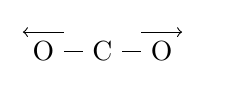
\begin{tikzpicture}
\useasboundingbox (-0.2,-0.2) rectangle (2,0.3);
%\draw (-0.2,-0.2) rectangle (2,0.3);

\draw  (0,0) node (o1) {O};
\draw  (0.75,0) node (c) {C};
\draw  (1.5,0) node (o2) {O};

\draw (o1) -- (c) -- (o2);
\draw[->] (o1.north east) -- (o1.north west);
\draw[<-] (o2.north east) -- (o2.north west);
\end{tikzpicture}
\end{marginfigure}
  $\bar{\nu} = 1337$~cm$^{-1}$. Hierbei ändert sich das Dipolmoment nicht, die Schwingung ist also nicht IR aktiv, wäre im Spektrum also nicht zu sehen.


\item[Asymmetrische Streckschwingung]
\begin{marginfigure}
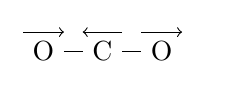
\begin{tikzpicture}
\useasboundingbox (-0.2,-0.2) rectangle (2,0.3);
%\draw (-0.2,-0.2) rectangle (2,0.3);

\draw  (0,0) node (o1) {O};
\draw  (0.75,0) node (c) {C};
\draw  (1.5,0) node (o2) {O};

\draw (o1) -- (c) -- (o2);
\draw[<-] (o1.north east) -- (o1.north west);
\draw[<-] (o2.north east) -- (o2.north west);
\draw[->] (c.north east) -- (c.north west);
\end{tikzpicture}
\end{marginfigure}
 $\bar{\nu} = 2349$~cm$^{-1}$. Hierbei ändert sich das Dipolmoment, die Schwingung ist also  IR aktiv.

\item[Biegeschwingung] 
\begin{marginfigure}
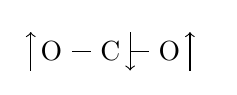
\begin{tikzpicture}
\useasboundingbox (-0.3,-0.2) rectangle (2,0.3);
%\draw (-0.2,-0.2) rectangle (2,0.3);

\draw  (0,0) node (o1) {O};
\draw  (0.75,0) node (c) {C};
\draw  (1.5,0) node (o2) {O};

\draw (o1) -- (c) -- (o2);
\draw[<-] (o1.north west) -- (o1.south west);
\draw[<-] (o2.north east) -- (o2.south east);
\draw[->] (c.north east) -- (c.south east);
\end{tikzpicture}
\end{marginfigure}
 $\bar{\nu} = 667$~cm$^{-1}$. Hierbei ändert sich das Dipolmoment, die Schwingung ist also  IR aktiv. Diese Mode ist zweifach entartet, da sie auch in der Ebene senkrecht zum Papier schwingen könnte. Für die Biegung ist das Potential weicher, die Frequenz daher niedriger als für die Streckung.
\end{description}


\paragraph{Wasser} Ein nicht-lineares Molekül mit $f=9 - 6 = 3$ Schwingungsfreiheitsgraden
\begin{description}
\item[Symmetrische Streckschwingung] 
\begin{marginfigure}
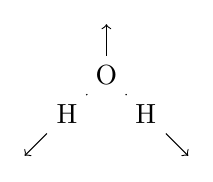
\begin{tikzpicture}
\useasboundingbox  (-0.5,-0.5) rectangle (1.5,1.1);
%\draw (-0.5,-0.5) rectangle (1.5,1.1);

\draw  (0,0) node (h1) {H};
\draw  (0.5,0.5) node (o) {O};
\draw  (1,0) node (h2) {H};

\draw (h1) -- (o) -- (h2);
\draw[->] (h1.south west) -- ++(-135:4mm);
\draw[->] (h2.south east) -- ++(-45:4mm);
\draw[->] (o.north) -- ++(up:4mm);
\end{tikzpicture}
\end{marginfigure}
  $\bar{\nu} = 3657$~cm$^{-1}$. Hierbei ändert sich das Dipolmoment, die Schwingung ist also  IR aktiv.

\item[Symmetrische Streck-Biegeschwingung]
\begin{marginfigure}
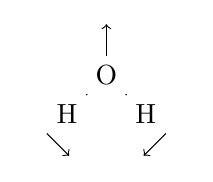
\begin{tikzpicture}
\useasboundingbox  (-0.5,-0.5) rectangle (1.5,1.1);
%\draw (-0.5,-0.5) rectangle (1.5,0.75);

\draw  (0,0) node (h1) {H};
\draw  (0.5,0.5) node (o) {O};
\draw  (1.,0) node (h2) {H};

\draw (h1) -- (o) -- (h2);
\draw[->] (h1.south west) -- ++(-45:4mm);
\draw[->] (h2.south east) -- ++(-135:4mm);
\draw[->] (o.north) -- ++(up:4mm);
\end{tikzpicture}
\end{marginfigure}
  $\bar{\nu} = 1595$~cm$^{-1}$. Hierbei ändert sich das Dipolmoment, die Schwingung ist also  IR aktiv.

\item[Asymmetrische Schwingung]
\begin{marginfigure}
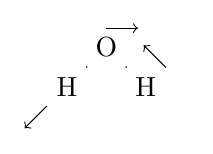
\begin{tikzpicture}
\useasboundingbox  (-0.5,-0.5) rectangle (1.5,0.75);
%\draw (-0.5,-0.5) rectangle (1.5,0.75);

\draw  (0,0) node (h1) {H};
\draw  (0.5,0.5) node (o) {O};
\draw  (1.,0) node (h2) {H};

\draw (h1) -- (o) -- (h2);
\draw[->] (h1.south west) -- ++(-135:4mm);
\draw[->] (h2.north east) -- ++(135:4mm);
\draw[->] (o.north) -- ++(east:4mm);
\end{tikzpicture}
\end{marginfigure}
  $\bar{\nu} = 3756$~cm$^{-1}$. Hierbei ändert sich das Dipolmoment, die Schwingung ist also  IR aktiv.
  
  
\end{description}

\paragraph{Cyanwasserstoff (Blausäure, HCN)}  
\begin{marginfigure}
\inputtikz{\currfiledir fig_hcn_modes}
\end{marginfigure}
Ein lineares Molekül mit $f=9 - 5 = 4$ Schwingungsfreiheitsgraden, analog zu Kohlendioxid oben. Das Spektrum am Anfang des Kapitels zeigt die Biegeschwingung bei $\bar{\nu} = 712$~cm$^{-1}$.  Abbildung \ref{fig:vib_hcn_all} gibt einen Überblick über einen größeren Spektralbereich. Man sieht zusätzlich den 
ersten Oberton der Biegeschwingung bei ungefähr der doppelten Frequenz  $\bar{\nu} = 1415$~cm$^{-1}$
. Die Mode bei  $\bar{\nu} = 3312$~cm$^{-1}$ ist die  asymmetrische Streckschwingung. Die symmetrische Streckschwingung  bei $\bar{\nu} = 2114$~cm$^{-1}$.
 Im Gegensatz zu \ch{CO2} bewegt sich in dieser Mode das Kohlenstoffatom ebenfalls, da die Massen von H und N verschieden sind, und sich ansonsten der  Schwerpunkt bewegen würde. Dies macht diese Mode sehr schwach IR-aktiv.  Nur für den Grundton der Biegeschwingung und die  symmetrische Streckschwingung ist der Q-Zweig erlaubt.

\begin{figure}
\inputtikz{\currfiledir fig_hcn-lowres}
\caption{Infrarot-Absorptionsspektrum von HCN Gas  (\cite{Maki_1995_HCN} via \href{https://hitran.org}{hitran.org}). Im unteren Spektrum ist ein größerer Ausschnitt bei geringer Auflösung gezeigt. Hier sind von den Rotationsbanden nur die Einhüllenden zu erkennen.
\label{fig:vib_hcn_all}}
\end{figure}



%%%%%%%%%%%%%%%%%%%%%%%%%%%%%%%%%%%%%%%%
%%%%%%%%%%%%%%%%%%%%%%%%%%%%%%%%%%%%%%%%



\section{Ziele}

\begin{itemize}
\item Sie können die Raman-Streuung im Dipol-Modell und als inelastische Streuung an einem virtuellen Zustand erklären.

\item Sie können das Raman-Spektrum einfacher Moleküle wie das untenstehende erklären und daraus Eigenschaften der Rotation und Vibration sowie des Kernspins berechnen.

\end{itemize}

\begin{figure}
\inputtikz{\currfiledir fig_n2_raman}
\caption{Raman-Spektrum von \ch{N2} in der Atmosphäre gemessen mit einem Laser der Wellenlänge 354.8~nm. Im Q-Zweig überlappen viele Linien, die hier nur als graue Fläche dargestellt sind. Daten aus \cite{Liu14_OE_N2}. }
\end{figure}


\section{Wie misst man das?}

Moleküle ohne permanentes Dipolmoment (also beispielsweise homonukleare Moleküle) zeigen im THz-Absorptionsspektrum kein Rotationsspektrum. Moleküle ohne  Variation des Dipol-Moments mit der Normal-Koordinate zeigen kein Vibrationsspektrum im Infraroten. Solche
Moleküle sind trotzdem spektroskopierbar, nämlich über den Raman-Effekt.

Der Raman-Effekt\sidenote{nach Chandrasekhara Venkata Raman, 1888--1970} ist die \emph{inelastische} Streuung von Licht an Materie, bei der sich also die Frequenz des Lichts ändert. Dies ist im Gegensatz zur Rayleigh-Streuung, die die \emph{elastische} Streuung von Licht beschreibt. Nur wenige Photonen werden inelastisch gestreut. Der Effekt ist daher mit dem Auge nicht wahrzunehmen und man benötigt eine spektral schmale und intensive Lichtquelle, also einen Laser. Diesen scheint man auf bzw. durch die Probe.\sidenote{Wir diskutiere hier Raman-Spektroskopie an Gasen. Raman-Streuung an festen Proben wird aber ebenfalls sehr oft zur Charakterisierung von Materialien eingesetzt.} Im Gegensatz zu den Spektroskopie-Methoden, die wir bisher betrachtete haben, wird hier das Licht \emph{senkrecht zur Stahlrichtung} detektiert. So misst man nur gestreutes Licht, nicht direkt den Laser. In einem hochauflösenden Spektrometer findet man dann bei drei Frequenzbereichen Photonen
\begin{itemize} \setlength{\itemsep}{0pt}
\item bei der Laser-Frequenz $\bar{\nu}_\text{laser}$. Dies ist die elastische Rayleigh-Streuung.
\item bei $\bar{\nu} < \bar{\nu}_\text{laser}$ inelastisch unter Energieverlust  gestreutes Licht. Dies nennt man Stokes-Linie. Sie ist etwa $10^{5}$ mal schwächer als die Rayleigh-Linie.
\item bei $\bar{\nu} > \bar{\nu}_\text{laser}$ inelastisch unter Energiegewinn gestreutes Licht. Dies nennt man Anti-Stokes-Linie. Sie ist noch einmal $10$ bis $100$ mal schwächer als die Stokes-Linie.
\end{itemize}
Die hier als Stokes- bzw. Anti-Stokes-Linie bezeichneten 'Linien' besitzen eine deutliche Struktur, sehr analog zu den Rotations-Vibrations-Spektren und beinhalten die gleiche Information über das Molekül.


\section{Klassische Erklärung des Schwingungs-Raman-Effekts}

Wir beginnen mit einer klassischen, makroskopischen Erklärung des Raman-Effekts. Das Molekül habe kein permanentes Dipolmoment, sei aber polarisierbar mit der Polarisierbarkeit $\alpha$. Zunächst vernachlässigen wir auch Rotation und Vibration des Moleküls. Dann ist das induzierte Dipolmoment
\begin{equation}
p_\text{ind}(t) = \alpha E(t) = \alpha E_0 \cos \omega_0 t \quad .
\end{equation}
Das Dipolmoment oszilliert also mit der Lichtfrequenz $\omega_0$. Laut den Maxwell-Gleichungen strahlen bewegte Ladungen elektromagnetische Felder ab, so auch dieses oszillierende Dipolmoment. Dies ist die Rayleigh-Streuung. Genauere Rechnungen zeigen, dass die Intensität proportional zu $\omega^4$ ist. Der Himmel ist also blau, weil blaues Licht besser Rayleigh-Streuung macht.

Nun erlauben wir die Vibration des Moleküls. Die Polarisierbarkeit hängt dann, bei passenden Molekülen, vom Kern--Kern--Abstand $R$ ab. Dies nähern wie in einer Taylor-Reihe
\begin{equation}
\alpha = \alpha(R) = \alpha(R_0) + \left. \frac{\partial \alpha}{\partial R} \right|_{R_0}  \left( R - R_0 \right) + \dots \quad .
\end{equation}
Der Kern--Kern--Abstand $R$ ändert sich periodisch mit der Schwingungs-Frequenz $\omega_\text{vib}$ und der Amplitude $q$, also
\begin{equation}
\left( R - R_0 \right) = q \, \cos \omega_\text{vib} t \quad .
\end{equation}
Nun berechnen wir analog zu oben das induzierte Dipolmoment
\begin{align}
p_\text{ind}(t) = & \alpha(t) E(t) \\
= & \alpha(R_0) E_0 \cos(\omega_0 t) +
\left. \frac{\partial \alpha}{\partial R} \right|_{R_0}   q \,  E_0 \, \cos (\omega_\text{vib} t)  \cos(\omega_0 t) \\
= & \underbrace{  \alpha(R_0) E_0 \cos(\omega_0 t) }_\text{Rayleigh} \\
& + \left. \frac{\partial \alpha}{\partial R} \right|_{R_0}  \frac{ q \,  E_0 }{2} 
\Bigl\{ 
\underbrace{ \cos \left( [\omega_0 -\omega_\text{vib}] t \right)}_\text{Stokes}  +  \underbrace{\cos \left( [\omega_0 + \omega_\text{vib}] t \right)  
}_\text{Anti-Stokes} 
\Bigr\}  \quad .
\nonumber
\end{align}
Das durch das oszillierende Dipolmoment abgestrahlte elektromagnetische Feld liefert wieder die Rayleigh-, jetzt aber auch die Stoks- und Anti-Stokes-Linie.

Allgemein gilt, auch nach 'moderner' Rechnung, dass Schwingungsmoden dann Raman-aktiv sind, wenn die  Polarisierbarkeit von $R$ abhängt, also 
\begin{equation}
\left. \frac{\partial \alpha}{\partial R} \right|_{R_0} \neq 0 \quad .
\end{equation}
Dies ist in zweiatomigen Molekülen \emph{immer} der Fall. In mehr-atomigen Molekülen \emph{mit Inversionssymmetrie} sind Raman-Aktivität und IR-Aktivität komplementär. Ein Beispiel dazu ist \ch{CO2}. Die symmetrische Streckschwingung ist nicht Infrarot-aktiv, aber im Raman-Spektrum sichtbar. Die asymmetrische Streckschwingung verhält sich genau umgekehrt.


\section{Mikroskopische Überlegungen}

Beim Raman-Prozess wechselwirken zwei Photonen mit dem Molekül, das einfallende und das auslaufende. Die quantenmechanische Beschreibung benötigt deshalb eine Störungstheorie zweiter Ordnung. Dies geht hier zu weit, ist aber beispielsweise in Kapitel 17 von \cite{Haken_wolf_II} dargestellt. Hier betrachten wir nur qualitative Argumente, die zumindest das Amplitudenverhältnis zwischen Stokes und Anti-Stokes-Linie erklären können. Diese sind nach obigen klassischen Überlegungen ja noch gleich stark.

Atome und Moleküle haben in der Quantenmechanik diskrete Energieniveaus. Photonen passender Frequenz können dann absorbiert werden. In der schematischen Darstellung verbindet ein senkrechter Pfeil zwei Niveaus.

\begin{marginfigure}
\begin{tikzpicture}
\begin{scope}
\draw[line width=1pt] (0,0) -- (1,0);
\draw[line width=1pt] (0,2) -- (1,2);
\draw[->] (0.5,0) -- (0.5,2);
\end{scope}
\begin{scope}[xshift=2cm]
\draw[line width=1pt] (0,0) -- (1,0);
\draw[line width=1pt, dashed] (0,2) -- (1,2);
\draw[->] (0.5,0) -- (0.5,2);
\end{scope}
\end{tikzpicture}
%\caption{Rotations-Vibrations-Übergänge liefert die P, Q, R-Zweige im Spektrum.}
\end{marginfigure}
 

Was passiert mit Photonen unpassender Frequenz? Diese können nicht absorbiert werden, dies würde schließlich die Energieerhaltung verletzten, aber sie werden gestreut. In der schematischen Darstellung zeichnet man dazu einen virtuellen Zustand als strichlierte horizontale Linie an das Ende des 'Photon'-Pfeils. Virtuelle Zustände können nicht bevölkert werden. Es gibt sie ja nicht wirklich. Auf der anderen Seite gibt es die Energie--Zeit--Unschärfe
\begin{equation}
\Delta E \cdot \Delta t \ge \hbar \quad .
\end{equation}
Wenn die Zeitdauer $\Delta t $ nur klein genug ist, dann muss die Energie-Unschärfe $\Delta E $ sehr groß werden. Für sehr kurze Zeiten kann man sozusagen gar nicht wissen, ob das Photon die passende Energie hat. Das kann man quantenmechanisch korrekt mit der Dichtmatrix formulieren. Für uns reicht hier, dass auch 'unpassende' Photonen mit diskreten Niveaus in Atomen oder Molekülen wechselwirken können, wenn auch nur für sehr kurze Zeit, wenige Femtosekunden für sichtbares Licht.

\begin{marginfigure}
\inputtikz{\currfiledir lorentz_oszillator}
\caption{Der dispersive Anteil des Lorentz-Oszillators fällt langsamer ab als der absorptive. }
\end{marginfigure}
 

Ein zweiter Gesichtspunkt kommt vom Lorentz-Oszillator aus Kapitel \ref{chap:4_diel}. Wir können diskrete atomare Übergänge als Lorentz-Oszillator beschreiben. Die Absorptionslinie hat das eben die bekannte Lorentz-Form. Sie fällt sehr schnell ab, wenn $| \omega  - \omega_0 |$ groß wird. Der Oszillator hat aber auch einen dispersiven Anteil, der den Realteil des Brechungsindexes beschreibt. Dieser fällt viel langsamer ab als der absorptive. Fern von der Resonanz ist er also wichtiger. Wir können uns ein Atom / Molekül fern von der Resonanz als ein kleines Volumen mit einem etwas von Vakuum verschiedene Brechungsindex vorstellen, das aber nicht absorbiert. Solch eine Brechungsindex-Variation führt aber zu Streuung von Licht.

\begin{marginfigure}%[-50mm]
\inputtikz{\currfiledir fig_raman_states}
\caption{Stokes- und Anti-Stokes-Streuung über einen virtuellen Zustand (strichliert). Die spektrale Position de Rayleigh-Linie entspricht der des einfallenden Lasers.}
\end{marginfigure}
 

Nach diesen Vorüberlegungen können wir das Zustandsdiagramm für den Raman-Effekt zeichnen, wenn das Molekül mehrere äquidistante Schwingungszustände hat, die mit der Quantenzahl $\nu$ durchnummeriert sind. Der Abstand der Schwingungszustände $\hbar \omega_\text{vib}$ ist klein gegen die Energie des Photons $\hbar \omega_0$. Das Photon wird an einem virtuellen Zustand gestreut. Das dabei entstehende zweite Photon wird abgestrahlt und durch den Pfeil nach unten symbolisiert. Dieser Pfeil kann entweder auf den Ausgangszustand $\nu = 0$ zurück gehen. Das ist Rayleigh-Streuung. Oder er endet auf einem höheren Zustand und liefert die Stokes-Linien bei niedrigerer Energie. Die Anti-Stokes-Linien erhält man, wenn man nicht von $\nu = 0$ ausgeht, sondern von einem höheren Zustand, und dann aber bis auf $\nu = 0$ zurück fällt. Damit ist die Energie des auslaufenden Photons größer als die des einfallenden.



Damit lassen sich verschiedene Aspekte des Raman-Effekts erklären: er ist sehr schwach, weil zwei Photonen quasi gleichzeitig ($\Delta t \approx 1$~fs) wechselwirken müssen. Die Intensität der Linien ist proportional zur Besetzung der Ausgangs-Schwingungszustände, also entsprechend einem Boltzmann-Faktor
\begin{equation}
\frac{I_\text{anti-Stokes}}{I_\text{Stokes}} = 
\frac{N_{\nu = 1}}{N_{\nu = 0}} =
 e^{- \frac{\hbar \omega_\text{vib}}{k_b T}} \quad .
\end{equation}
Bei Vibrationsfrequenzen von etwa $1000$~cm$^{-1}$ und $k_B T \approx 200 $~cm$^{-1}$ bei Raumtemperatur ist das Intensitätsverhältnis also $e^{-5} \approx 1 /150$. Man kann das Verhältnis der Linien also als lokales Thermometer benutzen.

Die quantenmechanischen Rechnungen ergeben die selben Auswahlregeln wie für die Infrarot-Schwingungsspektroskopie, also 
\begin{equation}
 \Delta \nu = \pm 1 \quad \text{falls harmonisch, sonst} \quad \pm 1, \pm 2, \dots   \quad .
\end{equation}



\section{Der Rotations-Raman-Effekt}

Ähnlich zu molekularen Schwingungen findet sich auch die Rotation der Moleküle im Raman-Spektrum. Wir beginnen wieder mit dem klassischen Modell. Elektromagnetisches Feld $E(t)$ und induziertes Dipolmoment $p_\text{ind}(t)$ sind wie oben
\begin{equation}
p_\text{ind}(t) = \alpha(t) E(t) = \alpha(t) E_0 \cos \omega_0 t \quad . \label{eq:raman_pind_rot}
\end{equation}
In die Zeitabhängigkeit der Polarisierbarkeit $\alpha(t)$ bauen wir jetzt die Rotation ein. Dazu nehmen wir an, dass die Polarisierbarkeit anisotrop ist, sich also für zwei senkrecht aufeinander stehende Richtungen unterscheidet: $\alpha_\parallel \neq \alpha_\perp$. Bei einem sich mit der Kreisfrequenz $\omega_R$ drehenden Molekül ist die Polarisierbarkeit also
\begin{equation}
\alpha(t) = \alpha_0 + \Delta \alpha \cos ( 2 \omega_R t) \quad \text{mit} \quad \Delta \alpha = \alpha_\parallel - \alpha_\perp \quad .
\end{equation}
Der Faktor $2$ kommt daher, dass die Polarisierbarkeit des Moleküls bereits nach $180^\circ$ wieder in sich übergeht. Dies setzen wir wieder in Gl. \ref{eq:raman_pind_rot} ein und multiplizieren aus. Wir bekommen analog zu oben
\begin{align}
p_\text{ind}(t) = & \underbrace{  \alpha_0 E_0 \cos(\omega_0 t) }_\text{Rayleigh} \\
& +   \frac{ \Delta \alpha \,  E_0 }{2} 
\Bigl\{ 
\underbrace{ \cos \left( [\omega_0 -2 \omega_R] t \right)}_\text{Stokes}  +  \underbrace{\cos \left( [\omega_0 + 2 \omega_R] t \right)  
}_\text{Anti-Stokes} 
\Bigr\}  \quad .
\nonumber
\end{align}
Die Linien sind also bei der doppelten Rotationsfrequenz ober- oder unterhalb der Rayleigh-Linie. Quantenmechanische Rechnungen ergeben als Auswahlregeln entweder
\begin{equation}
\Delta J = 0 \quad \text{und falls} \quad  \Delta \alpha \neq 0 \quad  \text{dann auch} \quad \Delta J = \pm 2 \quad .
\end{equation}
Die Position der Linien in einem Rotations-Raman-Spektrum sind also
\begin{equation}
 \bar{\nu} =  \bar{\nu}_\text{laser} \pm B \left[ (J+2) (J+3) - J(J+1) \right] = 
 \bar{\nu}_\text{laser} \pm B \left[ 4J + 6 \right] \quad ,
\end{equation}
wobei das $+$ die Anti-Stokes-Banden und das $-$ die Stokes-Banden liefert. Der Abstand der äquidistanten Linien ist damit nicht mehr $2B$ wie im Fall des THz-Absorptions-Spektrums, sondern $4B$. Da $B$ klein gegenüber $\bar{\nu}_\text{laser} $ ist, ist ein reines Rotations-Raman-Spektrum messtechnisch aufwändig. Eine sehr schwache Linie muss in kleinem spektralen Abstand zur starken Rayleigh-Linie detektiert werden. Dies erfordert einen hochauflösenden und stark unterdrückenden Monochromator, quasi immer durch die Hintereinanderschaltung von zwei oder drei Monochromatoren zu einem Doppel- bzw. Trippel-Monochromator realisiert.

\begin{marginfigure}
\inputtikz{\currfiledir rot_vib_raman}
\caption{Rotations-Vibrations-Spektrum in Raman-Streuung. Alle gezeichneten Linien und Übergänge sind Stokes-Übergänge.  \label{fig:raman_rotvib}}
\end{marginfigure}




 \section{Rotations-Vibrations-Raman-Effekt}

Analog zum Rotations-Vibrations-Spektrum in Absorption lässt sich die kombinierte Anregung eines Rotations- und Schwingungsniveaus auch im Raman-Effekt beobachten. Abbildung \ref{fig:raman_rotvib} skizziert die beteiligten Zustände für die Stokes-Bande, also die Linien die niederenergetisch von der Rayleigh-Linie liegen. Die Linienpositionen sind 

\begin{equation}
 \bar{\nu} =  \bar{\nu}_\text{laser} \pm \bar{\nu}_\text{vib} \pm B \left[ 4J + 6 \right]  \quad .
\end{equation}
Das erste $\pm$ unterscheidet zwischen Stokes ($-$) und Anti-Stokes ($+$). Das zweite $\pm$ ist gerade andersrum als das Vorzeichen von $\Delta J$. Man beachte, dass die Sequenz von äquidistanten Rotations-Linien wieder mit dem Abstand $6B$ von der reinen Vibrationslinie  $\Delta J = 0$ beginnt. Ähnlich zum Absorptionsspektrum werden die Linien mit $\Delta J =-2$ als O-Zweig, die mit 
$\Delta J =+2$ als S-Zweig bezeichnet.

\begin{margintable}
\begin{tabular}{rccccc}
$\Delta J$ & -2 & -1 & 0 & 1 & 2 \\
Zweig & O & P & Q & R & S
\end{tabular}
\caption{Nomenklatur der Zweige bei Rotationsspektren. $\Delta J = \pm 1$ im Absorptionsspektrum, $\Delta J = \pm 2$ im Raman-Spektrum sichtbar.}
\end{margintable}



\section{Einfluss der Kernspins}

Man beobachtet, dass das Rotations-Raman-Spektrum von zweiatomigen Molekülen aus zwei identischen Atomen eine charakteristische Intensitätsmodulation der Linien zeigt. Die Abbildung am Anfang des Kapitels ist ein Beispiel. Die Ursache dafür ist der Kernspin. Das Interessante an diesem Effekt ist, dass hier die \emph{Statistik} des Kernspins eine Rolle spielt: Für Triplett-Zustände gibt es beispielsweise drei mal mehr Möglichkeiten als für Singulett-Zustände. Dies führt am Schluss zu der beobachteten Intensitätsmodulation, nicht der potentiell ebenso mögliche magnetische Einfluss des Kernspins, der die Hyperfeinaufspaltung in Atomspektren bewirkt.

\begin{margintable}

\begin{tabular}{cc}
Molekül & $J_\text{ungerade}$  : $J_\text{gerade}$  \\ \hline
\ch{^1H2} & 3:1 \\
\ch{^2H2} & 1:2 \\
\ch{^{14}N2} & 1:2 \\
\ch{^{16}O2} & 1:0 
\end{tabular}
\caption{Beispiele für beobachtete Amplitudenverhältnisse.}
\end{margintable}

Wir müssen hierzu Überlegungen zur Symmetrie der Wellenfunktion des Moleküls anstellen. Diese sind in \cite{Haken_wolf_II}, Kapitel 12.4, in \cite{Demtröder_molekuelphysik}, Kapitel 4.5.3 dargestellt. Mir gefällt allerdings am Besten die Herangehensweise von \cite{HertelSchulz-2}, Kapitel 15.7.6, der ich hier folge.


Atomkerne sind entweder Fermionen, haben also einen halbzahligen Spin, oder sie sind Bosonen, haben also einen ganzzahligen Spin. Für Fermionen muss die Gesamt-Wellenfunktion anti-symmetrisch unter Vertauschung sein, für Bosonen symmetrisch. Die Frage ist also, wie sich die einzelnen Komponenten der Wellenfunktion ändern, wenn wir die beiden Atomkerne im Molekül vertauschen. Um das zu entscheiden, vertauschen wir nicht die Atomkerne, sondern tauschen den ganzen Rest, was am Ende das gleiche bewirkt.

\begin{itemize}\setlength{\itemsep}{0pt}
\item Zunächst drehen wir das ganze Molekül um 180$^\circ$ um eine Achse senkrecht auf die Kern--Kern--Achse. Dies tangiert die Elektronen nicht, aber die Rotation der Kerne um ebenfalls diese Achse bringt einen Faktor $(-1)^J$, wobei $J$ die übliche Rotations-Quantenzahl ist.

\item Dann machen wir eine Punkt-Spiegelung nur der Elektronen am Mittelpunkt des Moleküls. Das bewirkt einen Faktor $-1$ auf die Gesamt-Wellenfunktion, wenn der Gesamt-Zustand aller Elektronen ungerade ist, also ein $u$ im tiefgestellten Index hat.

\item Danach Spiegeln wir das Elektronensystem an einer Ebene, die die Kern--Kern--Achse beinhaltet. Das Ergebnis dieser Operation ist im hochgestellten Index $\pm$ im elektronischen Gesamt-Zustand angegeben.

\item Schließlich müssen wir noch die beiden Kernspins vertauschen. Die Symmetrie dieser Operation hängt von genauen Spinzustand ab und unterscheidet sich beispielsweise zwischen Singulett und Triplett.
\end{itemize}

\begin{marginfigure}[-50mm]
\inputtikz{\currfiledir swap_nucleus}
\caption{Eine Folge von Symmetrie-Operationen bewirken das Tauschen der Kerne, nach \cite{HertelSchulz-2}. Die Ellipse symbolisiert die Elektronen-Wellenfunktion, deren Orientierung durch den dickeren Teil angezeigt wird.}
\end{marginfigure}

 
 
Nach dieser Operationen haben wir effektiv die beiden Kerne vertauscht. Die Symmetrie ergibt sich damit aus dem Produkt der einzelnen aufgeführten Faktoren. Für Kerne mit ganzzahligem Spin, also Bosonen, muss die Gesamt-Wellenfunktion symmetrisch sein, also ein $+1$ am Ende der Rechnung herauskommen. In vielen Fällen sind dabei alle Parameter fest, bis auf die Rotations-Quantenzahl $J$ und der Spin-Zustand der Kerne. Beide bedingen sich dadurch gegenseitig. Wenn jeder einzelne Kern die Kernspin-Quantenzahl $I_1$ hat, dann kann die Gesamt-Kernspin-Quantenzahl $I$ zwischen $0$ und $2 I_1$ liegen. Für jedes $I$ gibt es $2 I +1$ Realisierungen mit unterschiedlichem $M_I$. Insgesamt gibt dies $(2 I_1 + 1)^2$ Möglichkeiten. Von diesen sind $(2 I_1 +1)( I_1 +1)$ symmetrisch und $(2 I_1 +1) I_1$ antisymmetrisch. Das Verhältnis der statistischen Gewichte $g$ beträgt also
\begin{equation}
 \frac{g_\text{symmetrisch}}{g_\text{anti-symmetrisch}} = \frac{I_1 + 1}{I_1} \quad .
\end{equation}
Dadurch ist die  'Geradheit' von $J$ mit einem unterschiedlichen statistischen Gewicht verknüpft.




\paragraph{Beispiel \ch{^1H2}} Jeder Kern hat $I = 1/2$, ist also ein Fermion und die Gesamt-Wellenfunktion muss anti-symmetrisch unter Vertauschen der beiden Kerne sein. 
Der elelktronische Grundzustand ist $^1\Sigma_g^+$, die beiden elektronischen Symmetrie-Operationen ändern also das Vorzeichen nicht.
Die Kernspin-Wellenfunktion kann sein
\begin{itemize}
\item \emph{anti-symmetrisch}, also $I = 0$. Damit die Symmetrie insgesamt anti-symmetrisch bleibt, muss der Rotationsanteil symmetrisch sein, also $J = \text{gerade}$. Dies nennt man \emph{para-Wasserstoff} und hat das statische Gewicht 1.

\item \emph{symmetrisch}, also $I = 1$. Damit die Symmetrie insgesamt anti-symmetrisch wird, muss der Rotationsanteil anti-symmetrisch sein, also $J = \text{ungerade}$. Dies nennt man \emph{ortho-Wasserstoff} und hat das statische Gewicht 3.
\end{itemize}
%
Da die Auswahlregeln $\Delta J = 2$ bei Raman-Übergängen verlangen, sind Übergänge ohne Änderung des Spins in einem Sub-System möglich. Es gibt im Wasserstoff-Molekül \ch{^1H2} also zwei Sätze von Linien, gerade und ungerade $J$, wobei die ungeraden um den Faktor 3 intensiver sind.




\paragraph{Beispiel \ch{^{16}O2}} Jeder Kern hat $I_1 = 0$, ist also ein Boson und die Gesamt-Wellenfunktion muss symmetrisch unter Vertauschen der beiden Kerne sein.  Der elektronische Grundzustand ist $^3\Sigma_g^-$, die Spieglung an der Ebene tauscht also das Vorzeichen. Der Gesamt-Kernspin kann nur ein symmetrischer Zustand mit $I = 0$ sein. Damit die Gesamt-Wellenfunktion symmetrisch bleibt, muss die Rotations-Wellenfunktion anti-symmetrisch sein, also $J = \text{ungerade}$. In Sauerstoff-Molekül  \ch{^{16}O2} fehlen also die Rotationslinien mit geradem $J$ vollständig. Wenn man den Kernspin nicht berücksichtigen würde, dann würde man eine doppelt so große Rotationskonstante $B$ annehmen.

%%%%%%%%%%%%%%%%%%%%%%%%%%%%%%%%%%%%%%%%
%%%%%%%%%%%%%%%%%%%%%%%%%%%%%%%%%%%%%%%%




\section{Ziele}

\begin{itemize}
\item Sie können die Struktur der optischen Absorptions- und Emissions-Spektren von Chromophoren wie die unten gezeigten erklären.

\item Sie können aus den gemessenen Spektren die Parameter des Bindungspotentials bestimmen, insbesondere die Frequenz der dominierende Schwingungsmode und die Änderung des Bindungsabstands im elektronisch angeregten Zustand.

\end{itemize}


\begin{figure}
\inputtikz{\currfiledir fig_bodipy}
  \caption{Absorptions- und Fluoreszenz-Spektrum des Farbstoffs BODIPY  (\href{https://www.thermofisher.com/de/de/home/life-science/cell-analysis/labeling-chemistry/fluorescence-spectraviewer.html?SID=srch-svtool&UID=10001moh}{thermofischer.com}).}
\end{figure}



\section{Überblick}

Von den in Kapitel \ref{chap:4_diel} diskutierten Formen der Anregung von Molekülen haben wir bis hier die Rotationsanregung mit der Quantenzahl $J$ und die Schwingungsanregung mit der Quantenzahl $\nu$ diskutiert. Nun kommt die ebenfalls schon in Kapitel  \ref{chap:4_diel} angesprochene elektronische Anregung hinzu. Es kann sich nun also auch die Wellenfunktion der Elektronen ändern. Die Gesamtenergie ist die Summe über die Energie in der Rotation, der Vibration und der im elektronischen System. Bei optischen Übergängen, also der Absorption und Emission von Licht, ändern sich damit potentiell diverse Quantenzahlen. Allerdings sind die drei Beiträge energetisch sehr unterschiedlich. Wenn der elektronische Anteil erfasst werden soll, dann können die anderen beiden nicht und nicht vollständig aufgelöst werden.\sidenote{Die relative Auflösung eines Spektrometers liegt im Bereich von etwa $10^{-4}$.} Insbesondere die Rotationsstruktur erscheint zu 'Banden' zusammengefasst.



\section{Wie misst man das?}


Es ist hilfreich, sich zu überlegen, wie das Lichtspektrum wirklich gemessen wird. Ein Lichtstrahl wird gebeugt, typischerweise an einem Gitter. Als Funktion des Dispersionswinkels misst man die Lichtintensität, indem man Photonen in Elektronen umwandelt, entweder in einer CCD-Kamera oder einer Photodiode. Die Signalamplitude ist also proportional zur Photonenrate, nicht zur Leistung oder zur Energie pro Photon.

Die Auflösung eines Gitterspektrometers wird durch die Breite der CCD-Pixel, die Größe der Diode oder des Eingangsspalts, durch die Größe eines monochromatischen Fokus oder einer Kombination aus allen bestimmt. In allen Fällen ist sie jedoch über das Spektrum konstant, wenn es in der Wellenlänge gemessen wird. Die natürliche Einheit eines Gitterspektrometers ist die Wellenlänge, nicht die Frequenz. Die reziproke Beziehung zwischen Wellenlänge und Frequenz führt zu 
\begin{equation}
 \Delta \nu = \nu_2 - \nu_2 = \frac{c}{\lambda_2} - \frac{c}{\lambda_1}  = c \frac{\lambda_1 - \lambda_2}{\lambda_1 \lambda_2} \approx \frac{c}{\lambda^2} \, \Delta \lambda \quad .
\end{equation}
Im Frequenzbereich ist die spektrale Auflösung also nicht konstant, sondern proportional zu $\nu^2$. Bei der Konvertierung eines Datensatzes vom Wellenlängenbereich in den Frequenzbereich werden also nicht nur die $x$-Werte, sondern auch die $y$-Werte konvertiert. Das Integral oder die Gesamtzahl der Photonen muss gleich bleiben.
\begin{equation}
 \left( \lambda \, ; \, F(\lambda) \right) \, \rightarrow  \left( \nu = \frac{c}{ \lambda} \, ; \,  F(\nu) = \frac{\lambda^2}{ c } \, F(\lambda) \right)  \quad .
\end{equation}
Dieses Problem tritt nur bei Lichtspektren auf. Absorptionsspektren sind das Verhältnis zweier Lichtspektren, des Signal- und des Referenzstrahls. In diesem Fall heben sich die Vorfaktoren auf und es müssen nur die $x$-Werte umgerechnet werden. Die spektral integrierte Absorption hat im Gegensatz zum spektral integrierten Photonenfluss keine Bedeutung.



\section{Vibronische Kopplung}

In Kapitel \ref{chap:vib} hatten wir die Born-Oppenheimer-Näherung eingeführt. Sie ermöglicht, die Elektronen- und die Kern-Wellenfunktionen zu separieren, da die Kernbewegung 'langsam' verglichen mit der Elektronen-Bewegung ist. Die Kerne bewegen sich also in einem gemittelten Potential der sich bewegenden Elektronen. Die Eigen-Energie des elektronischen Systems hängt von der Position der Kerne als Parameter ab.

Die Absorption eines Photons ändert \emph{instantan} die Wellenfunktion der Elektronen. Damit sehen die Kerne eine plötzliche Änderung des Potentials, in dem sie sich bewegen. Dies führt dann (bis auf sehr seltene Ausnahmen) zu einer Änderung der Bewegung der Kerne selbst, also eine Änderung der Rotations- und insbesondere der Schwingungs-Wellenfunktion bzw. deren Quantenzahlen. Dies nennt man vibronische Kopplung, also eine Kopplung zwischen der Vibration und den Elektronen.

Je nach Ausgangs- und Ziel-Wellenfunktion der Elektronen ändert sich der Gleichgewichtsabstand $R_0$ des Bindungspotentials,  die Energie $E(R_0)$ an diesem 
Abstand sowie die Form des Bindungspotentials $E(R- R_0)$. Typischerweise  sind angeregte Elektronenzustände weniger stark bindend, also $R_0$ ist größer, und weicher, also $E(R- R_0)$ ist breiter. Es gibt aber auch Ausnahmen von dieser Regel.
Und natürlich ist $E(R_0)$ höher, sonst wäre es ja keine Anregung.

\section{Franck-Condon-Prinzip}


Auch für die elektronische Anregung gibt es Auswahlregeln, die wieder durch das Übergangs-Matrixelement bestimmt werden. Man sieht wieder das einfallende elektromagnetische  Feld als Störterm und benutzt Fermis Goldene Regel. Gesucht ist dann das Übergangs-Matrixelement $D$
\begin{equation}
 D = \braket{\Psi_\text{final} | \hat{\mu} | \Psi_\text{initial} }
\end{equation}
zwischen den beiden Zuständen $\Psi_{f,i}$ und mit dem Dipol-Operator $ \hat{\mu}$. Die Born-Oppenheimer-Näherung erlaubt es nun, die Wellenfunktionen von Elektronen $ \phi(\mathbf{r}, \mathbf{R})$ und Kern $ \chi(\mathbf{R}) $ zu separieren:
\begin{equation}
 \Psi = \chi(\mathbf{R}) \, \phi(\mathbf{r}, \mathbf{R}) \quad , \label{eq:elec_wf_FC}
\end{equation}
wobei die Kern- ($\mathbf{R}$) und Elektronen-Koordinaten ($\mathbf{r}$) jeweils die Koordinate von \emph{allen} Elektronen und Kernen beinhalten und die Kern-Koordinaten $\mathbf{R}$ in der elektronischen Wellenfunktion nur fixer Parameter sind. Damit ist das Übergangs-Matrixelement $D$
\begin{equation}
 D =  \iint  \chi_f(\mathbf{R}) \, \phi_f(\mathbf{r} , \mathbf{R}) \; \hat{\mu}
 \,  \chi_i(\mathbf{R}) \, \phi_i(\mathbf{r}, \mathbf{R}) \, d \mathbf{r} \, d \mathbf{R}  \quad .
\end{equation}


Wir teilen den Dipol-Operator $\hat{\mu}$ jetzt auf in einen Teil, der nur auf die Position der negativen Ladungen, also der Elektronen wirkt, und einen Teil, der nur auf die Position der positiven Ladungen, also der Kerne wirkt
\begin{equation}
\hat{\mu} = \hat{\mu}_e + \hat{\mu}_k = q_e \mathbf{r} + q_k \mathbf{R} \quad .
\end{equation}
Damit erhalten wir
\begin{align}
D = & \braket{ \chi_f, \phi_f  |  \hat{\mu}_e |  \chi_i \phi_i} 
+ \braket{ \chi_f, \phi_f  |  \hat{\mu}_k |  \chi_i \phi_i}  \\
= & \braket{\chi_f | \chi_i} \,  \braket{ \phi_f  |  \hat{\mu}_e |   \phi_i} 
+ \braket{\phi_f | \phi_i} \,
\braket{ \chi_f |  \hat{\mu}_k |  \chi_i }   \quad .
\end{align} 
Im zweiten Schritt haben wir angenommen,  dass die Elektronen-Wellenfunktion $ \phi(\mathbf{r}, \mathbf{R})$  nur schwach von $\mathbf{R}$ abhängt. Die  Elektronen-Wellenfunktionen $\phi_i$ sind orthogonal zueinander. Der zweite Summand verschwindet also. Der Vorfaktor vor dem ersten ist nicht Null, weil die Kern-Wellenfunktionen zu verschiedenen Gleichgewichtsabständen gehören. Diesen Faktor 
\begin{equation}
 F =  \braket{\chi_f | \chi_i} =
 \int  \chi_f(\mathbf{R})  \,  \chi_i(\mathbf{R}) \, d \mathbf{R} 
\end{equation}
nennt man \emph{Franck-Condon-Faktor}. Er beschreibt den räumlichen Überlapp der Schwingungs-Wellenfunktion von Ausgangs- und Zielzustand. Da die Übergangsrate proportional zu $|D|^2$ ist, bestimmt sein Betrags-Quadrat die Intensität des Übergangs. 



Es macht intuitiv Sinn, dass ein solcher Faktor existieren muss. Bei einer elektronischen Anregung ändert sich die Elektronenwellenfunktion instantan. Die Position von  Teilchen mit Masse kann sich aber nicht instantan ändern.  Damit ein Übergang stattfinden kann, muss es also möglich sein, dass die Kerne auch im angeregten Zustand an diesem Ort sind. Das Franck-Condon-Integral berechnet gerade diese Möglichkeit.\sidenote{Dass sich die Position der Elektronen nicht ändert, wird analog durch $ \braket{ \phi_f  |  \hat{\mu}_e |   \phi_i} \neq 0 $ gefordert.}

Schematisch ist das in der Skizze gezeigt. Der Ausgangszustand für die Absorption eines Photons ist der elektronische Grundzustand und auch der Schwingungs-Grundzustand $\nu = 0$. Typische Schwingungs-Frequenzen sind so, dass $\hbar \omega_\text{vib} \gg k_b T$, also schon $\nu =1$ nicht thermisch angeregt werden kann. Das Bindungspotential im angeregten Zustand ist entlang der Kern-Kern-Koordinate $R$ nach außen verschoben (weniger stark bindend). Seine Form ist näherungsweise gleich zum Grundzustand. 

\begin{marginfigure}
   \inputtikz{\currfiledir FC_vib_state_wf}
\caption{Die Absorption eines Photons führt zur Anregung der Kern--Kern--Schwingung, wenn die Potentiale gegeneinander verschoben sind.}
\end{marginfigure}

Wir hatten die Schwingungs-Wellenfunktionen $\chi_f(\mathbf{R})$ bereits in Kapitel \ref{chap:vib} besprochen. Für harmonische Potentiale sind es Hermite'schen Polynomen. Im elektronischen Grundzustand ist der Kern-Kern-Abstand $R$ also stark um $R_0$ lokalisiert. Direkt nach der elektronischen Anregung kann sich $R$ aber nicht geändert haben. Optische Übergänge sind \emph{senkrecht} in dieser Skizze. Wir suchen also eine Schwingungs-Wellenfunktion bzw. deren Quantenzahl $\nu$ im angeregten elektronischen Zustand, die möglichst viel Aufenthaltswahrscheinlichkeit bei $R_0$ hat (aber auch die Geschwindigkeit der Kerne muss übereinstimmen). Im Beispiel ist dies $\nu = 1$. Den Grad der Übereinstimmung gibt der Franck-Condon-Faktor an.

Es gibt damit also keine scharfen Auswahlregeln, nur mehr oder weniger starke Übergänge bei gegebenen $\nu_\text{final}  = \Delta \nu$. Falls sich der Bindungsabstand überhaupt nicht ändert unter der elektronischen Anregung, dann ist der Übergang
\begin{equation}
 \nu = 0 \rightarrow \nu = 0
\end{equation}
der stärkste. Diesen Übergang nennt man 'zero phonon line' (ZPL), weil keinerlei Schwingungsquanten involviert sind\sidenote{Das Konzept der Phononen wird im Teil zur Festkörperphysik behandelt}. Je größer der Unterschied in $R_0$, desto weiter verschiebt sich die stärkste Linie zu höheren $\nu$. 



\section{Franck-Condon-Prinzip im harmonischen Potential}

\begin{marginfigure}[0mm]
   \inputtikz{\currfiledir fig_parabola}
\caption{Der Kopplungsterm $-A R$ im Potential des angeregten Zustandes $e$ verschiebt das Minimum der Parabel zu größeren Werten von $R$ und niedrigeren Werten des Potentials. }
\end{marginfigure}

Anhand des harmonischen Potentials wollen wir dies etwas genauer betrachten. Ein Molekül mit einem elektronischen Grundzustand $g$ und einem elektronischen angeregten Zustand $e$ kann periodische Schwingungen der Kernpositionen entlang einer Koordinate $R$ erfahren. 
Wir nehmen an\footcite{Kuzmany}, dass das Potential dieser Schwingungen harmonisch ist, also
\begin{eqnarray}
 U_g(R) &=& \frac{1}{2} \, K \, R^2 = \frac{1}{2} \, M \, \Omega^2 \, R^2 \\
  U_e(R) &=&  U_g(R) + E_{eg} - A \, R = E_{eg}  - A \, R + \frac{1}{2} \, M \, \Omega^2 \, R^2  \quad ,
 \end{eqnarray}
wobei $E_{eg}$ der elektronische Beitrag zur Energiedifferenz ist. Wir nehmen an, dass beide Potentiale die gleiche Form, d.h. die gleiche Schwingungsfrequenz haben. Der Term $A \, R$ koppelt den elektronischen Zustand und die Kernbewegung. Er verschiebt das Potential des angeregten Zustands entlang der $R$-Koordinate. 
%
Wir führen eine reduzierte Raumkoordinate $\tilde{R}$ ein
\begin{equation}
\tilde{R} = \frac{R}{x} \quad \text{mit} \quad x = \sqrt{\frac{\hbar}{M \Omega}}  \quad .
\end{equation}
Die neue Raumkoordinate $\tilde{R}$ ist so skaliert, dass die Parabel des Potentials die Energie des Schwingungs-Grundzustands $\hbar \Omega/2$ bei $\tilde{R} = 1$ schneidet.
In diesen Koordinaten liegt das Minimum der Parabel des Grundzustands weiterhin bei 
$\tilde{R}  = 0$, das des
angeregten Zustands bei $\tilde{R} = \tilde{R}_e$ mit
\begin{equation}
\tilde{R}_e = \frac{A \, x}{ \hbar \Omega} \quad .
\end{equation}
In diesen Koordinaten sind die Potentiale also
\begin{eqnarray}
 U_g(\tilde{R}) &=& \frac{1}{2}  \, \hbar \Omega \, \tilde{R}^2 \\
  U_e(\tilde{R}) &=&   E_{eg} + \frac{1}{2}  \, \hbar \Omega  \, \left[  (\tilde{R} - \tilde{R}_e)^2 - \tilde{R}_e^2  \right]
 \end{eqnarray}
Die Energien der quantenmechanischen Eigenzustände sind 
\begin{eqnarray}
  E_{g, n} &=&  (n + 1/2) \, \hbar \Omega  \\
  E_{e, m} &=&   E_{eg} +   (m + 1/2 - \tilde{R}_e^2  /2 ) \, \hbar \Omega  =  E_{eg} +   (m + 1/2 - S ) \, \hbar \Omega   \nonumber
\end{eqnarray}
wobei wir den  Huang-Rhys-Faktor $S$ als dimensionslose Kopplungskonstante eingeführt\sidenote{Kuzmany definiert  $S$ als Wurzel des hier verwendeten $S$.}  haben
\begin{equation}
 S = \frac{1}{2} \, \tilde{R}_e^2  =
 \frac{A^2}{\hbar \Omega}  \, \frac{1}{2 M \Omega^2} \quad. 
\end{equation}
Der  Huang-Rhys-Faktor $S$ ist also ein Maß für die Verschiebung des Bindungspotentials im angeregten Zustand.



Die Eigenfunktionen $\chi_n$ der Kernvibrationen sind Hermite'sche Polynome. Der Franck-Condon-Faktor beschreibt das Überlappungsintegral der Schwingungswellenfunktion von Grund- und angeregtem Zustand. Da der elektronische Übergang im Vergleich zur Kernbewegung schnell ist, kann sich die Kernkoordinate während des Übergangs nicht ändern (Born-Oppenheimer-Näherung), und sowohl der Grund- als auch der angeregte Zustand benötigen eine nicht verschwindende Wahrscheinlichkeit, um auf der gleichen Koordinate $r$ zu liegen. Wenn sich einer der Zustände in einem schwingenden Grundzustand befindet, d.h. $n$ oder $m$ gleich null ist, nimmt der Franck-Condon-Faktor die Form\sidenote{Diese Notation ist schlampig in dem Sinne, dass die Bra-Wellenfunktion ein elektronischer angeregter Zustand ist, die Ket-Funktion ein elektronischer Grundzustand!}
\begin{equation}
 | \braket{ \chi_0 | \chi_m } | ^2  =  | \braket{ \chi_m | \chi_0 } | ^2 = \frac{S^m \exp(-S)}{m!} 
\end{equation}
was eine Poisson-Verteilung des Mittelwertes $S$ ist.  Der stärkste Übergang ist also der Übergang in $m \approx S$, der bei großer Kopplung zwischen elektronischem und nuklearem System, d.h. großem $S$, vom 0--0 Übergang abweicht.

\begin{figure}
  \inputtikz{\currfiledir fig_poisson}
  \caption{Poisson-Verteilungen}
\end{figure}

%Der Debye-Waller-Faktor $D$ gibt das Verhältnis der kohärent gestreuten Welle zu allen Streuprozessen an. Bei Molekülen entspricht dies der Amplitude der 0--0-Linie zum Integral über die gesamte Bande. Da die Summe über alle Franck-Condon-Faktoren zum gleichen Endzustand eins ist, erhalten wir
%\begin{equation}
% D =  | \braket{ \chi_0 | \chi_0 } | ^2 = \exp(-S)
%\end{equation}

\section{Spin-Auswahlregeln und Termschema}

Der elektronische Teil der Wellenfunktion in Gl. \ref{eq:elec_wf_FC} kann wie immer noch weiter unterteilt werden in seinen räumlichen Anteil $\phi^\text{Raum}$ und in den Spin-Anteil  $\phi^\text{Spin}$. Der Dipol-Operator $\hat{\mu}$ interagiert nicht mit dem Spin-Anteil. Somit lässt sich das Übergangs-Matrix-Element schreiben als
\begin{equation}
 D =   \braket{\chi_f | \chi_i} \,    \braket{\phi^\text{Spin}_f | \phi^\text{Spin}_i}  \,
  \braket{\phi^\text{Raum}_f | \hat{\mu} | \phi^\text{Raum}_i}  \quad .
\end{equation}
Da die Spin-Wellenfunktionen orthogonal aufeinander sind, dürfen sich bei einem optischen Übergang die Spin-Quantenzahlen nicht ändern, also
\begin{equation}
 \Delta S = 0 \quad .
\end{equation}
Übergänge finden nur innerhalb eines 'Systems' statt, also nur zwischen  Singulett-Zuständen und nur zwischen   Triplett-Zuständen.
Störungen wie beispielsweise die Spin-Bahn-Kopplung können diese Regel aufweichen. Man spricht dann von 'intersystem crossing'.

In Kapitel \ref{chap:MO-teil2} hatten wir die Termschema zur Bezeichnung der Elektronen-Orbitale in der Form  $^3\Sigma_g^- $ eingeführt. Dies war in dieser Form nur für zweiatomige Moleküle möglich. Allgemein bezeichnet man die Zustände daher mit S für Singulett und T für Triplett und nummeriert sie mit der Energie aufsteigend durch. Der Grundzustand ist typischerweise ein Singulett, also S0. Fluoreszenz ist der Übergang S1 nach S0. Der Übergang T1 nach S0 ist Spin-verboten. Dies bedeutet aber nur, dass die Übergangsrate von etwa 1/ns auf 1/\textmu s bis 1/s abfällt. Solche Strahlung nennt man Phosphoreszenz. Lumineszenz ist der Oberbegriff für beides. 

Unter Umständen überlappen hoch angeregte Schwingungsniveaus eines elektronisch niedrigen Zustands mit niedrigen Schwingungsniveaus eines höher angeregten Zustands gleicher Multiplizität\sidenote{gleicher Spin-Quantenzahlen}. In solchen Fällen kann der höhere elektronische Zustand in den niedrigeren übergehen. Diesen Prozess nennt man 'internal conversion'.


\section{Fluoreszenz}

Fluoreszenz bezeichnet den Prozess, in dem ein Photon von einem Molekül emittiert wird. Dabei geht das Molekül von einem angeregten elektronischen Zustand in einen niedrigeren Zustand über. Der Prozess wird durch die selben Franck-Condon-Faktoren bestimmt und auch hier sind die Übergänge 'senkrecht', also bei unverändertem Kern-Kern-Abstand $R$.

Allerdings ist die Kopplung der Elektronen an das Lichtfeld ein schwacher Prozess. Dies hat bei der Absorption keinen besonderen Einfluss. Wenn kein Photon absorbiert wird, dann passiert eben nichts und das Molekül verbliebt weiter im Grundzustand mit $\nu = 0$. Vor der Emission ist das Molekül allerdings potentiell in einem Zustand mit $\nu > 0$. In einem solchen Fall kann das Molekül Energie abgeben und in den Schwingungs-Grundzustand des elektronisch angeregten Zustand relaxieren. Die Energie geht in diesen Fällen entweder an die Umgebung oder an andere Schwingungsmoden des Moleküls. In jedem Fall sind diese strahlungslosen Übergänge hin zu $\nu = 0$ etwa um den Faktor 1000 schneller als die Emission eines Photons\sidenote{1 Prozess pro 1 ps vergleichen mit 1 Prozess pro 1 ns}. Fluoreszenz-Emission geschieht daher immer aus dem Zustand $\nu = 0$. Dies ist die Regel von Kasha.

\section{Spiegelregel}

In Kombination mit den zwischen Absorption und Emission identischen Franck-Condon-Faktoren führt  Kashas Regel dazu, dass das Fluoreszenz-Spektrum wie das an der zero-phonon line gespiegelte Absorptionsspektrum aussieht\footcite[Kapitel 1.3.2 und 1.3.3]{Lakowicz2010}. Wenn eine Schwingung mit der Frequenz $\omega$ das Spektrum dominiert, dann liegen die Peaks im Spektrum bei
\begin{align}
  E_{abs, n} = & E_{00} + n \, \hbar \omega \\
  E_{fl, n} = & E'_{00} - n \, \hbar \omega \quad .
\end{align}
Die Energie der zero phonon line $E_{00}$ ist zunächst einmal in Absorption und Emission identisch.  Hinzu kommt aber ggf. noch die Stokes-Verschiebung, wenn sich beispielsweise Lösemittel-Moleküle in der Umgebung des fluoreszierenden Moleküls umorientieren, je nach dem in welchem elektronischen Zustand das emittierende Molekül ist.



Nicht nur die spektralen Positionen, sondern auch die Amplitude der Peaks im Absorptionsspektrum $A(\omega)$ und Fluoreszenzspektrum $F(\omega)$ stehen in Beziehung zueinander. Der Grund dafür ist, dass die Einstein-Koeffizienten $A_{12}$ und $B_{21}$ miteinander verwandt sind, oder dass es nur ein Übergangs-Dipolmoment $\mu$ gibt, das sowohl die Absorption als auch die Emission bestimmt. Man muss allerdings die Beziehung zwischen dem Übergangsdipolmoment $\mu$ und den Spektren beachteten \footcite[Kapitel 5.2]{Parson}
\begin{eqnarray}
   A(\omega  )  & \propto & \omega_{g,m \rightarrow e,n}  \,  \left| \braket{\chi_n |  \chi_m} \right|^2 
\,  \left| \braket{\phi^\text{Raum}_e | \hat{\mu} | \phi^\text{Raum}_g} \right|^2 \\
   F(\omega ) & \propto & \omega_{e,n \rightarrow g,m}^3 \,  \left| \braket{\chi_m |  \chi_n} \right|^2 
\,  \left|\braket{\phi^\text{Raum}_g | \hat{\mu} | \phi^\text{Raum}_e} \right|^2 \quad .
\end{eqnarray}
Eigentlich ist das spektrale Integral über eine Linie in $A(\omega  )$ bzw. $F(\omega)$ mit einem Übergang und damit einem Franck-Condon-Faktor verbunden. Das Integral hat man unter der Annahme einer Linienform aufgelöst. Dabei verbleibt ein Faktor $\omega$ auf der rechten Seite von beiden Gleichungen. Das Fluoreszenzspektrum erhält einen zusätzlichen Faktor von $\omega^2$ aufgrund der optischen Modendichte im dreidimensionalen Raum, wie es im Schwarzkörperspektrum und in der  Beziehung zwischen den Einstein-Koeffizienten $A_{12}$ und $B_{12}$ auftritt.
Alles zusammengenommen sollte man daher $A / \omega$ und $F / \omega^3$ vergleichen.


\section{Stokes-Verschiebung}

Vergleicht man Absorptions- und Emissionsspektren wie oben beschrieben, so stellt man fest, dass die Übergangsenergien 0--0 nicht vollständig übereinstimmen. Dies ist die Stokes-Verschiebung. Ihre Amplitude hängt vom Molekül und der Umgebung des Moleküls ab. Wenn ein Molekül in einen elektronisch angeregten Zustand überführt wird, ändert sich die räumliche Verteilung der Elektronendichte. Dies beeinflusst die Umgebung, z. B. die Lösungsmittelmoleküle, in Position und Orientierung. Unmittelbar nach der Anregung befinden sich die Lösungsmittelmoleküle noch in der Position, die im Grundzustand des Farbstoffmoleküls die geringste Energie liefert. Im angeregten Zustand verschieben sie sich und richten sich neu aus, um die Gesamtenergie zu verringern. Die Fluoreszenzemission findet also in einer anderen elektrischen Umgebung statt als die Absorption, was zu einer Verschiebung der Übergangsenergie, der Stokes-Verschiebung, führt.

Allgemeiner  wird nicht nur der Unterschied zwischen den 0--0-Übergängen, sondern auch der Unterschied zwischen den Spitzen der Absorptions- und Emissionsspektren als Stokes-Verschiebung bezeichnet. Dazu gehört dann auch die Schwingungsrelaxation des Farbstoffmoleküls selbst.



\section{Elektronische Spektren großer Moleküle}

Große Moleküle mit vielen Kernen und Elektronen besitzen komplexe Spektren in den optischen Übergängen, insbesondere bei hochauflösender Spektroskopie in der Gasphase\sidenote{In diesem Fall kann man die Doppler-Verbreitungen nicht vernachlässigen bzw. muss ihren Einfluss eliminieren.}. Man kann die beobachteten Spektren aber grob nach der Art, dem Ursprung der angeregten Elektronen klassifizieren.

\paragraph{Bindende Elektronen} Wenn Elektronen angeregt werde, die besonders relevant für eine Bindung sind, dann führt dies oft zur Dissoziation, also dem Aufbrechen des Moleküls. Das Bindungspotential im elektronisch angeregten Zustand ist dann entweder selbst nicht mehr bindend, oder hat beispielsweise über die Schwingungszustände großen Überlapp mit einem anderen nicht-bindenden Potential. Dissoziation geschieht also nicht durch den direkten Übergang gebunden--frei, sondern über einen Zwischenschritt.

\paragraph{Chromophore Gruppen} Ein Chromophor ist ein Farb-Träger. Manche Elektronen-Orbitale zeigen charakteristische Eigenschaften unabhängig davon, wie diese in ein großes Molekül eingebaut sind. Wenn diese Orbitale dann zu Fluoreszenz-Emission führen, dann nennt man sie chromophore Gruppen. Ein Beispiel sind einzelne Atome von Übergangsmetallen (\ch{Fe}, \ch{Ti}, \ch{Co}). Diese zeigen nahezu atomare Spektren, auch wenn sie in größere Moleküle eingebaut sind. Ein anderes Beispiel ist die \ch{C=O} Doppelbindung oder die \ch{C=C} Doppelbindung. Diese haben ein charakteristisches Absorptionsspektrum bei einer Wellenlänge von 290 nm bzw. 180 nm, unabhängig vom Rest des Moleküls.

\paragraph{Delokalisierte Elektronen} Manchmal ist ein Elektronen-Orbital nicht eine Linearkombination von nur zwei Atom-Orbitalen, sondern es sind mehr Atome an dem Orbital beteiligt. Ein Elektron in einem solchen Orbital ist also nicht mehr an einem Ort, sondern über einen größeren Bereich delokalisiert. Wir hatten das in Kapitel  \ref{chap:MO-teil2} im Zusammenhang mit der Hückel-Methode besprochen. In Benzol beispielsweise wird die $\sigma$-Bindung aus den sp$^2$-Hybrid-Orbitalen aufgebaut. Die verbleibenden 6 Elektronen in den atomaren p$_z$-Orbitalen bilden ein delokalisiertes $\pi$-Elektronen-System, oft durch einen Kreis in der Mitte des 6-Rings dargestellt. Ein anderes Beispiel sind konjugierte Polymere, also alternierende Einfach- und Doppel-Bindungen in einer Kette von Kohlenstoffatomen. In solchen Fällen ist jedes beteiligte Elektron überall. Elektronen in einem solchen räumlich großen Orbital kann man ähnlich zu einem Teilchen im Kasten beschreiben. Das Orbital bildet das Kasten-Potential. Die Kettenlänge bestimmt die Kastenbreite und, da $E \propto 1 /L$, die Lage der Energieniveaus. Lange Moleküle absorbieren und emittieren röter.



\section{Zusammenfassung}

\textit{Schreiben Sie hier ihre persönliche Zusammenfassung des Kapitels auf. Konzentrieren Sie sich auf die wichtigsten Aspekte.}

\vspace*{10cm}


%--------------------
\printbibliography[segment=\therefsegment,heading=subbibliography]
